\documentclass[a4paper]{article}

%% Language and font encodings
\usepackage[english]{babel}
\usepackage[utf8]{inputenc}
\usepackage[T1]{fontenc}

%% Sets page size and margins
\usepackage[a4paper,top=3cm,bottom=2cm,left=3cm,right=3cm,marginparwidth=1.75cm]{geometry}

%% Useful packages
\usepackage{amsmath}
\usepackage{graphicx}
\usepackage[colorinlistoftodos]{todonotes}
\usepackage[colorlinks=true, allcolors=blue]{hyperref}
\usepackage{floatrow}
\usepackage{float}
\usepackage{subcaption}
\usepackage{booktabs}
\usepackage{color}
\usepackage{tikz}
\usepackage{caption}
\usetikzlibrary{shapes.geometric, arrows}

% package to manage citations
\usepackage[backend=bibtex,style=authoryear-comp,sorting=nyt,isbn=false,url=false, natbib=true]{biblatex}
\addbibresource{references.bib}

\tikzstyle{startstop} = [rectangle, rounded corners, minimum width=3cm, minimum height=1cm,text centered, draw=black,text width = 5cm, fill=red!30]
\tikzstyle{io} = [trapezium, trapezium left angle=70, trapezium right angle=110, minimum width=3cm, minimum height=1cm, text centered, draw=black, fill=blue!30]
\tikzstyle{process} = [rectangle, minimum width=3cm, minimum height=1cm, text centered, text width = 4cm, draw=black, fill=orange!30]
\tikzstyle{decision} = [diamond, minimum width=2cm, minimum height=1cm,text centered,text width = 2.5cm, draw=black, fill=green!30]
\tikzstyle{arrow} = [thick,->,>=stealth]

\definecolor{ErasmusBlue}{RGB}{12, 32, 116}

\begin{document}
\title{PRIAS Personalized Biopsy Schedules}

\author{Firstname1 Lastname1}

\date{}

\maketitle

% !TEX root =  ../main_manuscript.tex 
\begin{abstract}
\texttt{Background}: Prostate cancer active surveillance (AS) patients undergo repeat biopsies. Active treatment is advised when biopsy Gleason grade group~$\geq$~2 (\textit{upgrading}). Many patients never experience upgrading, yet undergo biopsies frequently. Personalized biopsy decisions based on upgrading-risk may reduce patient burden.\\

\texttt{Objective}: Develop a risk prediction model and web-application to assist patients/doctors in personalized biopsy decisions.\\

\texttt{Design, Setting, and Participants}: Model development: world's largest AS study PRIAS, 7813 patients, 1134 experienced upgrading; External validation: largest five cohorts of Movember Foundation's GAP3 database (${>20,000}$ patients, 27 centers worldwide); Data: repeat prostate-specific antigen (PSA) and biopsy Gleason grade.\\

\texttt{Outcome Measurements, and Statistical Analysis}: A Bayesian joint model fitted to the PRIAS dataset. This model was validated in GAP3 cohorts using risk prediction error, calibration, area under ROC (AUC). Model and personalized biopsy schedules based on predicted risks were implemented in a web-application.\\

\texttt{Results and Limitations}: Cause-specific cumulative upgrading-risk at year five of follow-up: 35\% in PRIAS, at most 50\% in GAP3 cohorts. PRIAS based model: PSA velocity was a stronger predictor of upgrading (Hazard~Ratio:~2.47, 95\%CI:~1.93--2.99) than PSA value (Hazard~Ratio:~0.99, 95\%CI:~0.89--1.11). Validation: Moderate AUC (0.55--0.75) in PRIAS and GAP3 cohorts. Moderate prediction error (0.1--0.3) in GAP3 cohorts where impact of PSA value and velocity on upgrading-risk was similar to PRIAS, but large (0.3--0.45) otherwise. Recalibration advised for external cohorts.\\

\texttt{Conclusions}: We successfully developed and validated a model for predicting upgrading-risk, and providing risk-based personalized biopsy decisions, in prostate cancer AS. The model made available via a web-application enables shared decision making of biopsy schedules by comparing fixed and personalized schedules on total biopsies and expected time delay in detecting upgrading.\\

\texttt{Patient Summary}: Personalized prostate biopsies are a novel alternative to fixed one-size-fits-all schedules. The underlying statistical models are made available through a user-friendly web-application and may help to reduce unnecessary prostate biopsies while maintaining cancer control.
\end{abstract}
% !TEX root =  ../main_manuscript.tex 
\section{Introduction}
Patients with low- and very low-risk screening-detected localized prostate cancer are usually advised active surveillance (AS) instead of immediate radical treatment~\citep{briganti2018active}. In AS, cancer progression is routinely monitored via prostate-specific antigen (PSA), digital rectal examination, and repeat biopsies. Among these, the strongest indicator of cancer-related outcomes is the biopsy Gleason grade~\citep{epsteinGG2014}. When the Gleason grade increases from grade~1 (Gleason 3+3) to 2 (Gleason 3+4) or higher, called \textit{reclassification}, patients are commonly advised curative treatment~\citep{bul2013active}.

\begin{figure}
\centerline{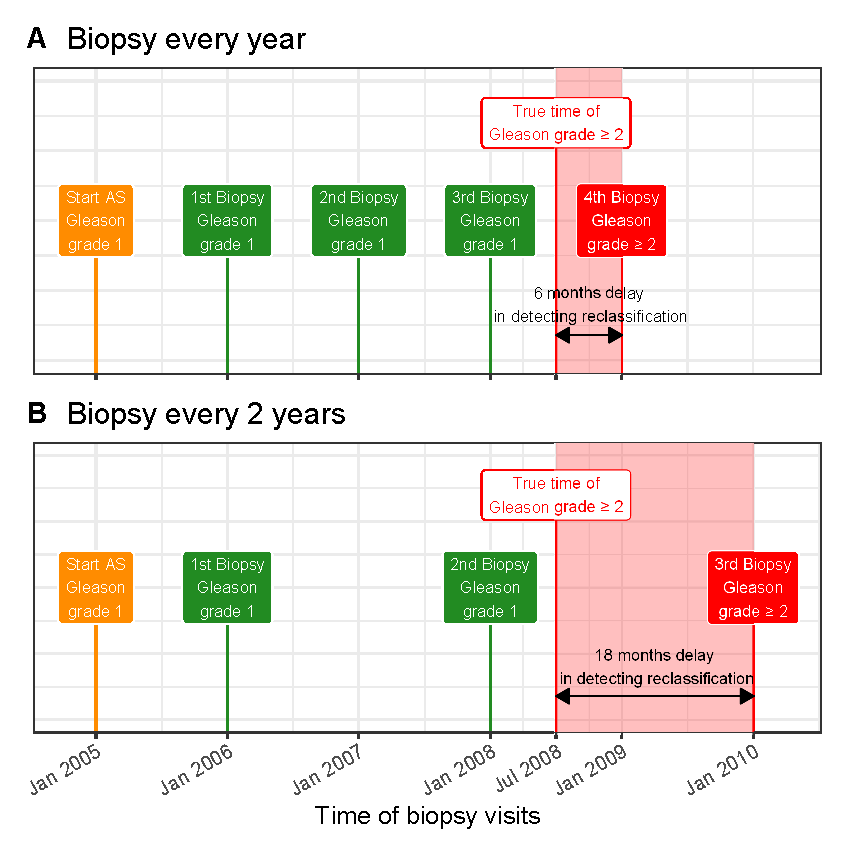
\includegraphics[width=\columnwidth]{images/delay_explanation.eps}}
\caption{\textbf{Trade-off between the number of biopsies and time delay in detecting reclassification (Increase in Gleason grade from 1 to 2 or higher):} The true time of reclassification for the patient in this figure is July 2008. When biopsies are scheduled annually (\textbf{Panel~A}), reclassification is detected in January 2009 with a time delay of six months, and a total of four biopsies are scheduled. When biopsies are scheduled biennially (\textbf{Panel~B}) reclassification is detected in January 2010 with a time delay of 18 months, and a total of three biopsies are scheduled. Since biopsies are conducted periodically, the time of reclassification is observed as an interval. For example, between Jan~2008--Jan~2009 in \textbf{Panel~A} and between Jan~2008--Jan~2010 in \textbf{Panel~B}.}
\label{fig:delay_explanation}
\end{figure}

Biopsies are conducted periodically. Consequently, reclassification is always detected with a time delay (Figure~\ref{fig:delay_explanation}). For detecting reclassification timely, many AS programs schedule fixed and frequent biopsies (e.g.,~annually) for all patients~\citep{nieboer2018active,loeb2014heterogeneity}. However, this also leads to many unnecessary biopsies in slow/non-progressing patients. Biopsies are invasive, painful and prone to medical complications. Thus, biopsy burden and patient non-compliance to frequent biopsies~\citep{bokhorst2015compliance} has raised concerns regarding the optimal biopsy schedule~\citep{inoue2018comparative, bratt2013study}. To this end, infrequent schedules such as biennial biopsies have been proposed as an alternative~\citep{inoue2018comparative,de2017estimating}. Although, biennial biopsies may still lead to five unnecessary biopsies over ten years (current study period of large AS programs) for slow/non-progressing patients. A promising alternative to fixed and frequent biopsies is personalized biopsy schedules based on the patient-specific risk of reclassification (Figure~\ref{fig:riskBasedExample}).

\begin{figure}
\centerline{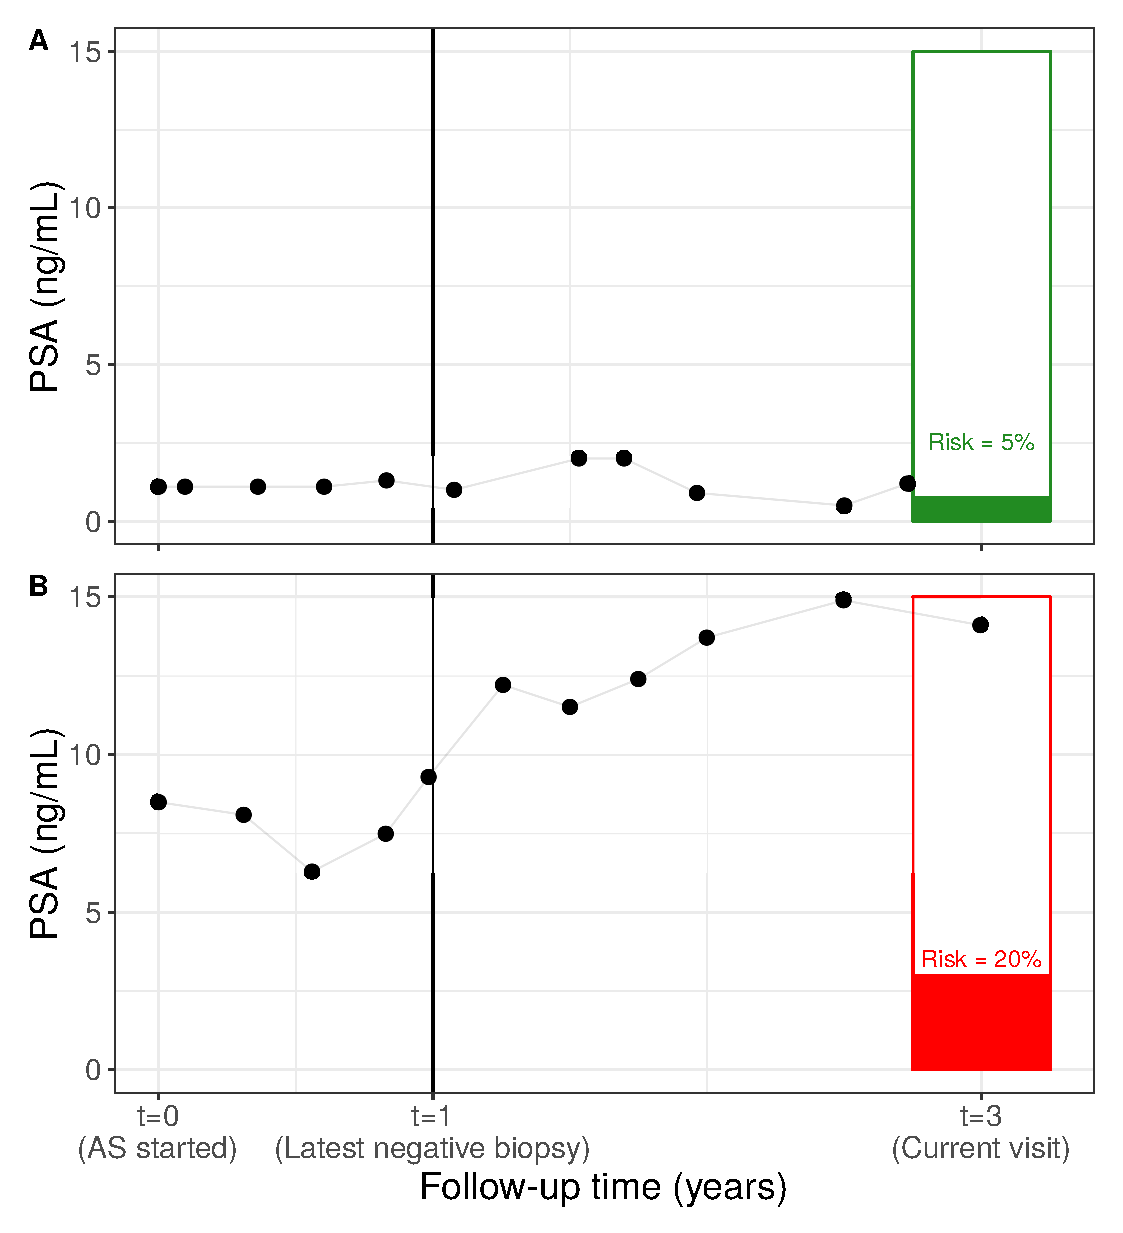
\includegraphics[width=\columnwidth]{images/riskBasedExample.eps}}
\caption{\textbf{Motivation for personalized risk-based decisions of biopsy}: Patient~A (\textbf{Panel~A}) and B (\textbf{Panel~B}) had their latest biopsy at year one of follow-up (green vertical line). Patient~A's prostate-specific antigen (PSA) profile remained stable until his current visit at year three, whereas patient~B's profile has shown a rise. Consequently, patient~B's estimated cumulative risk of reclassification at the current visit (year three) is higher than that of patient~A. This makes patient~B a more suitable candidate for biopsy than Patient~A. Risk estimates in this figure are only illustrative.}
\label{fig:riskBasedExample}
\end{figure}

The first challenge in developing personalized biopsy schedules is consolidating accumulated patient data (e.g., PSA, previous biopsy results) into risk estimates for reclassification. Existing calculators for risk of reclassification~\citep{partin1993use,makarov2007updated} use only the latest PSA measurement of a patient. In contrast, we intend to utilize all repeated measurements of PSA, previous biopsy results, and baseline characteristics of a patient. To this end, a suitable model is the joint model for time-to-event and longitudinal data~\citep{tomer2019, coley2017prediction,rizopoulos2012joint}. A joint model predicts risk of reclassification in a personalized manner. A subsequent challenge however, is translating risks into clinical decisions. For example, a 10\% risk of reclassification can be perceived high/low depending upon the patient age. Patients may also weigh risks of reclassification with the potential \textit{consequences} of another biopsy. Two relevant \textit{consequences} of biopsies (Figure~\ref{fig:delay_explanation}) are the timing and total number of biopsies (burden), and the time delay in detecting reclassification (smaller is beneficial). The relative importance of these \textit{consequences} can vary between the patients, and also over the follow-up period for the same patient.

The goal of this work was to assist patients and doctors in making better decisions of biopsies than fixed and frequent biopsies. For this purpose, we developed a web-application that gives patients their current and future risk of reclassification. It also suggests them risk-based personalized schedules of biopsies. For each biopsy schedule, be it fixed or personalized, the web-application provides expected \textit{consequences} of following it. Thus, patients can compare schedules before making a decision. The web-application uses a prediction joint model fitted to the world's largest AS dataset, PRIAS~\citep{bul2013active}. We externally validated this model in five largest AS cohorts of the GAP3 database \citep{gap3_2018}. Thus, the web-application can be used by a large number of patients worldwide.
% !TEX root =  ../main.tex 

\section{Joint model for Gleason reclassification and PSA levels}
\label{sec : jm_introduction}
The first step in creating a personalized schedule for biopsies is to come up with a model for Gleason scores, PSA levels and other subject specific characteristics. In PRIAS, PSA levels are measured at the time of induction, every 3 months for the first 2 years in the study and then every 6 months thereafter. Thus PSA levels can be modeled as a longitudinal outcome. As mentioned earlier, patients in PRIAS have a Gleason score of 6 or less at the time of induction in the study, and patients are removed from AS the first time Gleason reclassification takes place. Since our interest also lies in time to Gleason reclassification, we model it as a time to event outcome. i.e. time to Gleason reclassification. While univariate modeling of the two aforementioned outcomes can be done separately using longitudinal model and survival models, it is important to note that they are not independent. To model the association between the two types of outcomes we use a joint model for time to event and longitudinal outcomes.

\subsection{Definition}
Let $T_i^*$ denote the true Gleason reclassification time for the $i^{th}$ subject. Let the times at which biopsies are conducted for the $i^{th}$ patient be denoted by $C_i = \{C_{i0}, C_{i1}, ... C_{ig_i}; C_{ij} < C_{ik}, \forall j<k \}$. $T_i^*$ cannot be observed directly and it is only known that it falls in an interval $(l_i, r_i]$, where $l_i = C_{i(g_i-1)}, r_i = C_{ig_i}$ if Gleason reclassification is observed and $l_i = C_{ig_i}, r_i=\infty$ if patient drops out. The latter is also known as right censoring. Let $\boldsymbol{y}_i$ denote the $n_i \times 1$ longitudinal outcome vector for the PSA levels of the $i^{th}$ subject. The population of interest is all the patients enrolled in AS. For a sample of $n$ patients from this population the complete data is denoted by $\mathcal{D}_n = \{T_i, l_i, r_i, \boldsymbol{y}_i; i = 1,...n\}$, where $T_i \epsilon (l_i, r_i]$ denotes the observed time of Gleason reclassification.\\

To model the evolution of the longitudinal outcome, which is PSA levels in the case at hand, the joint model utilizes a linear mixed effects model. The longitudinal outcome $y_i(t)$ at time $t$ is modeled as:

\begin{equation*}
\begin{split}
y_i(t) &= m_i(t) + \varepsilon_i(t), \\
&= x_i^T(t) \beta + z_i^T(t) \boldsymbol{b}_i + \varepsilon_i(t)
\end{split}
\end{equation*}
%Do not introduce a space here, otherwise it starts a new paragraph
where, $m_i(t)$ denotes the true and unobserved value of the longitudinal outcome at time $t$. $\varepsilon_i(t) \sim N(0, \sigma^2)$ denotes the measurement error term, assumed normally distributed with variance $\sigma^2$. $\beta$ denotes the vector of the unknown fixed-effects parameters. $\boldsymbol{b}_i \sim N(0, \boldsymbol{D})$ denotes the vector of random effects, assumed normally distributed with mean zero and covariance matrix D, and independent of $\varepsilon_i(t)$. $x_i(t)$ and $z_i(t)$ denote row vectors of the design matrices for the fixed and random effects, respectively. For non continuous longitudinal outcomes joint models utilize Generalized linear mixed models \citep{rizopoulos2012joint}.\\

Since both PSA levels and Gleason scores are affected by the state of prostate cancer, they are inherently correlated with each other. To this end, the joint model utilizes a relative risk sub-model where the hazard of Gleason reclassification $h_i(t)$ at any time point $t$ depends on the history of true and unobserved values of PSA levels $\mathcal{M}_i(t) = \{m_i(s), 0\leq s \leq t\}$ measured up to that time point. Joint models offer flexibility in modeling this dependence. In its simplest form, the hazard may depend on instantaneous value of PSA $m_i(t)$ at time $t$. More sophisticated ones are dependence of hazard at time $t$ on PSA-DT, PSA velocity $m'_i(t) = \dfrac{d m_i(t)}{dt}$, or even on the cumulative effect of PSA $\int_0^t m_i(s) \,ds$ up to $t$. The fact that any functional form of dependence is possible, is evident from the following equation:

\begin{equation*}
h_i(t \mid M_i(t); \theta) = h_0(t) e^{\gamma^Tw_i + f\{M_i(t), \boldsymbol{b}_i, \alpha\}}
\end{equation*}
where $h_0(t)$ is the baseline hazard at time $t$. $w_i$ is a vector of time independent covariates and $\gamma$ are the corresponding parameters. The function $f(\cdot)$ parametrized by vector $\alpha$ specifies the features of longitudinal outcome that are are included in the linear predictor of the relative risk model.\\

While $\alpha$ controls the strength of association between the hazard of reclassification and features of the PSA levels, the fact that both Gleason scores and PSA levels are internally related to a patient's health, is manifested by the random effects $\boldsymbol{b}_i$ in the model. The joint model postulates that given the random effects, time to Gleason reclassification and PSA levels measured at different time points are mutually independent. As mentioned earlier, in PRIAS study PSA-DT is used to decide the schedule of biopsies. Although PSA-DT is computed using observed PSA values, dependence on observed longitudinal history $\mathcal{Y}(t) = \{y_i(s), 0\leq s \leq t\}$ at any time $t$, is not the same as dependence on patient's health. This because dependence on patient's health, manifested by $\boldsymbol{b}_i$ is same as dependence on future unobserved values of PSA. Thus the inference for the parameters of interest $\theta$ doesn't change even if uncertainty in biopsy schedule $C_i$ is not modeled. The kernel of the corresponding joint likelihood conditional on the random effects is given by:

\begin{equation*}
p(T_i, l_i, r_i, \boldsymbol{y}_i \mid \boldsymbol{b}_i; \theta) \propto p(T_i \mid l_i, r_i, \boldsymbol{b}_i; \theta) p(\boldsymbol{y}_i \mid \boldsymbol{b}_i; \theta)
\end{equation*}

\subsection{Fitting the joint model to PRIAS dataset}
One of the goals of this work is to compare various scheduling methods for patients of the PRIAS study. We also compare the scheduling methods using a simulation study. For both of these goals, we require parameter estimates of  the joint model between time to Gleason reclassification and PSA levels of PRIAS' patients. For the first goal the parameter estimates are used directly to schedule visits using personalized schedules. For the second goal, we require the parameter estimates of the  joint model to generate data for a simulation study. For these reasons and to also introduce constructs such as dynamic survival probability, we next fit a joint model to the PRIAS data set.\\

The PRIAS data set contains information about 5943 prostate cancer patients who satisfied the conditions for enrollment in AS. For every patient the age at the time of induction in AS was recorded. Other information, namely, PSA levels and Gleason scores were measured at different time points on the basis of a predetermined schedule as mentioned earlier in the report. For the longitudinal analysis of PSA measurements we used $\log_2(PSA + 1)$ measurements instead of the raw data. The log transformation was done because the PSA scores took very large values at the onset of disease progression. This indicated that the underlying distribution for PSA scores was right skewed. Secondly at certain time points patients' PSA scores were measured to be 0, and thus we had to add a constant 1 to all PSA scores before log transformation. We found the same transformation in literature as well \cite{mcgreevy2006impact,sene2016individualized}. For the variable Age in the Cox model, we wanted to  consider both the linear and quadratic effect. However doing so led many numerical instabilities while performing the joint model analysis. To avoid these pitfalls we had to center the Age variable around age 70 years. The longitudinal and survival submodels of the joint model we fitted is given by:

\begin{align*}
\log_2\{PSA + 1\}(t) &= m_i(t) + \varepsilon_i(t), \\
m_i(t) &= (\beta_0 + b_{i0}) + \beta_1 (Age-70) + \beta_2 (Age-70)^2\\ 
&+ \sum_{k=1}^4 \beta_{k+2} B_k(t,\mathcal{K}) + b_{i1} B_7(t, 0.5) + b_{i2} B_8(t, 0.5) \\
\varepsilon_i(t) & \sim N(0, \sigma^2),\\
\boldsymbol{b}_i & \sim N(0, \boldsymbol{D})
\end{align*}

The evolution of PSA levels over time is modeled flexibly using B-splines. For the fixed effects part the spline consists of 3 internal knots. The internal knots are at $\mathcal{K} =\{0.5, 1.2, 2.5\}$ years, and boundary knots are at 0 and 7 years. For the random effects part there is only 1 internal knot at 0.5 years and the boundary knots are at 0 and 7 years. The choice of knots was based on exploratory analysis as well as on the basis of model selection criteria AIC and BIC. For the survival submodel the hazard function we fitted is given by:

\begin{equation}
h_i(t) = h_0(t) e^{\gamma_1 (Age-70)  + \gamma_2 (Age-70)^2  \alpha_1 m_i(t) + \alpha_2 m'_i(t)}
\end{equation}

The baseline hazard $h_0(t)$ is modeled as in equation \ref{eq : baseline_hazard}. To fit the joint model we use the R package JMbayes \cite{rizopoulosJMbayes}, which uses a Bayesian approach for parameter estimation. The parameter estimates for the survival submodel were estimated using Bayesian ridge methodology.

\subsubsection{Parameter Estimates}
The parameter estimates for the joint model we fitted to the PRIAS data set are shown in Table \ref{tab : PSA_long} and Table \ref{tab : PSA_survival}. Since the longitudinal evolution of $\log_2(PSA + 1)$ is modeled with non-linear terms, the interpretation of the coefficients corresponding to time is not straightforward. In lieu of the interpretation we present the fitted evolution of PSA over a period of 10 years for a patient who is 70 years old in Figure \ref{fig : fitted_trend_psa}. It can be seen that the after the first 6 months the PSA levels steadily increase over the follow up period. Since the model for PSA has only additive terms, this evolution remains same for all patients. The effect of Age only affects the baseline PSA score. However it is so small that it can be ignored for all practical purposes.\\

\begin{figure}[!htb]
	\centering
    \captionsetup{justification=centering}
	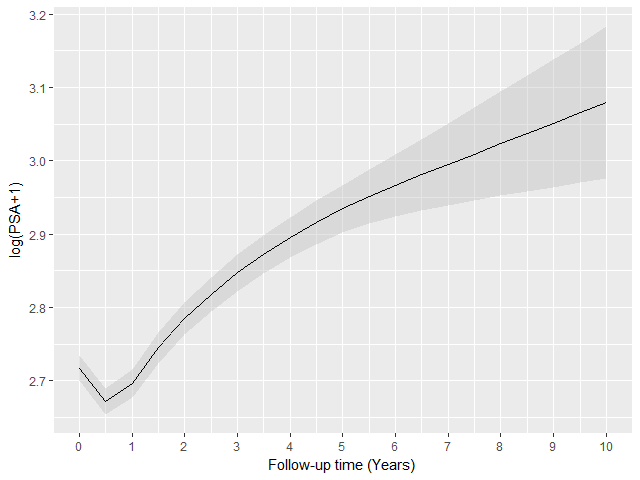
\includegraphics[width=0.8\textwidth]{fitted_trend_psa.png}
	\caption{Fitted evolution of $\log_2(PSA+1)$ over a period of 10 years, for a patient who was inducted in AS at the Age of 70 years.}
	\label{fig : fitted_trend_psa}
\end{figure}

\begin{table}[!htb]
\centering
\caption{Longitudinal submodel estimates for joint model.}
\label{tab : PSA_long}
\captionsetup{justification=centering}
\begin{tabular}{@{}lrrrrr@{}}
\toprule
                                     & Mean   & Std. Dev           & 2.5\%               & 97.5\%              & P              \\ \midrule
Intercept                            & 2.717  & 0.008              & 2.701               & 2.733               & \textless0.000 \\
(Age - 70)                           & 0.003  & 0.001              & 0.001               & 0.005               & 0.002          \\
(Age - 70) $\times$ (Age - 70)       & -0.001 & 1 $\times 10^{-4}$ & -7 $\times 10^{-4}$ & -4 $\times 10^{-4}$ & \textless0.000 \\
Spline: visitTimeYears{[}0, 0.5{]}   & 0.026  & 0.008              & 0.012               & 0.042               & \textless0.000 \\
Spline: visitTimeYears{[}0.5, 1.2{]} & 0.208  & 0.013              & 0.184               & 0.233               & \textless0.000 \\
Spline: visitTimeYears{[}1.2, 2.5{]} & 0.175  & 0.019              & 0.137               & 0.210               & \textless0.000 \\
Spline: visitTimeYears{[}2.5, 7{]}   & 0.309  & 0.028              & 0.256               & 0.366               & \textless0.000 \\
$\sigma$                               & 0.273  & 0.001              & 0.271               & 0.275               & \textless0.000 \\ \bottomrule
\end{tabular}
\end{table}

For the survival submodel, the parameter estimates in Table \ref{tab : PSA_survival} show that both the $\log_2(PSA + 1)$ value and $\log_2(PSA + 1)$ velocity are associated with time to Gleason reclassification. The effect is quite strong and if at any given time point the PSA becomes approximately 4 times of its value then the hazard of Gleason reclassification  becomes 1.5 times of the original. This is valid under the condition that the $\log_2(PSA + 1)$ velocity remains the same. The effect of $\log_2(PSA + 1)$ velocity is far stronger, but it is not interpretable easily. Lastly, for the effect of Age on hazard we can say that it can be safely ignored for all practical purposes.

\begin{table}[!htb]
\centering
\caption{Survival submodel estimates for joint model.}
\captionsetup{justification=centering}
\label{tab : PSA_survival}
\begin{tabular}{@{}lrrrrr@{}}
\toprule
Variable                      & Mean   & Std. Dev & 2.5\%  & 97.5\%                 & P              \\ \midrule
Age - 70                      & 0.036  & 0.007    & 0.023  & 0.050                  & \textless0.000 \\
(Age - 70) $\times$ (Age - 70) & -0.002 & 0.001    & -0.004 & 2 $\times 10^{-4}$ & 0.016          \\
$\log_2(PSA + 1)$                  & 0.184  & 0.093    & 0.016 & 0.369                  & 0.032          \\
Slope: $\log_2(PSA + 1)$           & 1.937  & 0.278    & 1.420  & 2.525                  & \textless0.000 \\ \bottomrule
\end{tabular}
\end{table}

\subsubsection{Dynamic survival probability}
\label{subsubsec: dyn_surv_prob}
Since patients' PSA levels and Gleason scores are periodically measured, the entire PSA and repeat biopsy history can be used to periodically update the predictions about about time to Gleason reclassification. More specifically, let us assume that a new patient numbered $j$, not present in the original sample of patients $\mathcal{D}_n$, did not have a Gleason reclassification at their last biopsy, performed at time $t$. Further, let us assume that the PSA measurements are available for the patient $j$ up to a time point $s > t$. Then combining these two pieces of information, the distribution for time to Gleason reclassification for this patient is given by:

\begin{equation}
p(T^*_j | T^*_j > t, \mathcal{Y}_j(s), \mathcal{D}_n; \theta^*)
\end{equation}

where $\mathcal{Y}_j(s) = \{y_j(r); 0 \leq r \leq s\}$ denotes the history of PSA measurements done up to time $s$. The personalized schedules we propose in this work depend on this dynamic distribution for time to Gleason reclassification. As more PSA measurements are taken and repeat biopsies are performed, this distribution is accordingly updated. The survival probabilities based on this distribution are called dynamic survival probabilities \cite{rizopoulos2011dynamic}. The dynamic survival probability at any time point $u > s$ is given by:

\begin{equation}
\pi_j(u|t) = Pr(T^*_j \geq u| T^*_j >t, \mathcal{Y}_j(s), D_n; \theta)
\end{equation}

\begin{figure}[!htb]
	\centering
    \captionsetup{justification=centering}
	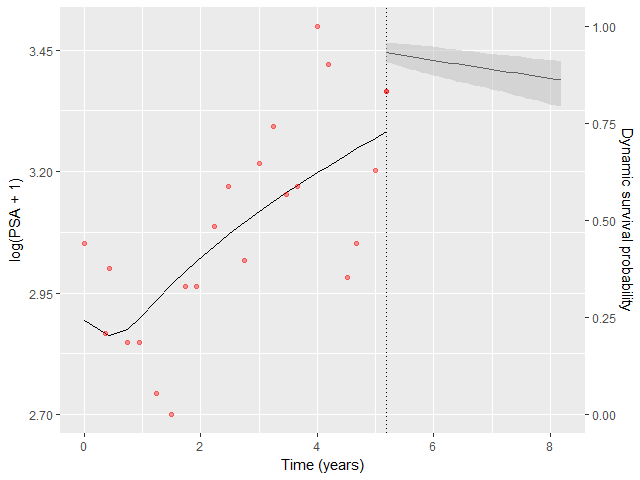
\includegraphics[width=0.8\textwidth]{dyn_surv_prob_2362.png}
	\caption{Dynamic survival probability for patient with ID 2362 in the PRIAS data set.}
	\label{fig : dyn_surv_prob_2362}
\end{figure}

As an example we present the dynamic survival probability of patient 2362 from the PRIAS data set. Patient 2362 had his last repeat biopsy at 3.78 years at which the Gleason reclassification did not happen. The patient was later censored at 5.12 years. Using all this information up to 5.12 years, the dynamic survival probability at any time point $u > 3.78$ for this patient is given by the formula $Pr(T^*_{2362} \geq u| T^*_{2362} > 3.78, \mathcal{Y}_{2362}(5.12), D_n; \theta)$. Figure \ref{fig : dyn_surv_prob_2362} shows the dynamic survival probability for patient 2362 at time points between 5.12 and 8.12 years.
\section{Personalized scheduling approaches}
\label{sec : personalized_scheduling}
Once a joint model for Gleason reclassification and PSA levels is obtained, the next step is to use it to create personalized schedules for biopsies. In this section we present the various personalized biopsy scheduling approaches and their motivation. The personalized schedules that we propose are dynamic in nature and thus at any given time, only 1 future biopsy is scheduled. The age of the patient and entire PSA, repeat biopsy history up to that time point is considered while computing the time of next biopsy. To elucidate the scheduling methods, we use patient $j$, introduced in detail in section \ref{subsubsec: dyn_surv_prob}, as a case.

\subsection{Conditional expected time to Gleason reclassification}
Given that the patient $j$ hadn't had Gleason reclassification up to time $t$, an estimate of true Gleason reclassification time, with zero bias and least squared loss is the conditional expected Gleason reclassification time: $E(T^*_j | T^*_j > t, \mathcal{Y}_j(s), D_n; \theta)$. The aforementioned two properties are also the motivation for using conditional expected Gleason reclassification time as the time of next biopsy. 

\begin{equation}
\label{eq : expectedFailureTime}
E(T^*_j | T^*_j > t, \mathcal{Y}_j(s), D_n; \theta) = t + \int_t^\infty \pi_j(u|t) \,du
\end{equation}

where, $\pi_j(u|t)$ is the dynamic survival probability (Section \ref{subsubsec: dyn_surv_prob}) for patient $j$ at time $u$. While expected time to Gleason reclassification is unbiased, it is more useful when the variance of time to Gleason reclassification, given by $Var(T^*_j | T^*_j >t, \mathcal{Y}_j(s), \mathcal{D}_n; \theta)$, is less. The variance is given by:

\begin{equation}
\label{eq : varFailureTime}
Var(T^*_j | T^*_j >t, \mathcal{Y}_j(s), \mathcal{D}_n; \theta) = 2 \int_t^\infty {(u-t) \pi_j(u|t) \,du} - {\bigg(\int_t^\infty \pi_j(u|t) \,du\bigg)}^2
\end{equation}

\subsection{Dynamic risk of failure}
\label{subsec : dynamic_risk_definitions}
When time to Gleason reclassification has a large variance (Eq. \ref{eq : varFailureTime}) then the offset (Section \ref{sec : introduction}) based on using conditional expected time to Gleason reclassification can vary wildly from patient to patient. In such a scenario a doctor/patient may want to perform biopsies earlier than the expected time to Gleason reclassification. This can be achieved by not crossing the risk of Gleason reclassification beyond a certain threshold.\\ 

The personalized scheduling approaches based on dynamic risk of reclassification, schedule biopsies at time points $u > t$ such that the dynamic risk of failure $1 - \pi_j(u|t)$ is higher than a certain threshold $1-\kappa$ beyond $u$. Or in other words the dynamic survival probability $\pi_j(u|t)$ is below a threshold $\kappa$ beyond $u$. The choice of the threshold $\kappa \epsilon [0,1]$ can be on the basis of amount of risk a patient or doctor is willing to take. It is also possible to automate the choice of $\kappa$. One such way is to choose a $\kappa$ for which a binary classification accuracy measure is maximized. In case of joint models, time dependent binary classification is more relevant because a patient can be in control group at some time $t_a$ and it can be in the cases at some future time point $t_b > t_a$. Based on \cite{rizopoulosJMbayes} we consider a subject $j$ to be a case if $\pi_j(t + \Delta t|t) \leq \kappa$ and a control if $\pi_j(t + \Delta t|t) > \kappa$. The time window $\Delta t$ can be either chosen on a clinical basis (such as 1 year in PRIAS) or it can be chosen at a point where $AUC(t, \Delta t)$ \cite{rizopoulosJMbayes} is largest. i.e. we chose a $\Delta t$ for which the model has the most discriminative capability at time $t$. Various binary classification accuracy measures can be maximized to select the cutoff $\kappa$. The ones we use in this report are:

\begin{itemize}
\item Max Sensitivity: $\underset{\kappa \epsilon [0, 1]} {\text{arg max Senstivity}}$,\\
where sensitivity is $P(\pi_j(t + \Delta t|t) \leq \kappa | T^*_j \epsilon (t, t + \Delta t])$ . 
\item Youden J Statistic: Sensitivity + Specificity - 1,\\
where the specificity is defined as $P(\pi_j(t + \Delta t|t) > \kappa | T^*_j > t + \Delta t)$.
\item Accuracy (ACC): $\dfrac{TP(t) + TN(t)}{TP(t) + FP(t) + TN(t) + FN(t)}$, where TP(t), FP(t), TN(t) and FN(t) are the number of true positives, false positives, true negatives and false negatives at time point $t$.
\item F1 Score: $\dfrac{2TP(t)}{2TP(t) + FP(t) + FN(t)}$, and it is derived by taking harmonic mean of precision and sensitivity.
\end{itemize}

We also compare $\kappa$ chosen by these automatic selection methods against a fixed $\kappa = 0.85$. The choice of 0.85 was arbitrary, assuming a scenario where a patient/doctor does not want to exceed 15\% risk of progression.

% !TEX root =  ../main.tex 

\section{Personalized schedules for patients in PRIAS}
\label{sec : pers_schedule_PRIAS}
As a first step in demonstrating how the personalized schedules work, we created a biopsy schedule for patients in PRIAS. To this end, we divided the PRIAS data set into training(5938 subjects) and demonstration data sets (5 subjects). We demonstrate that the biopsy schedule depend on subject specific traits and the evolution of PSA scores.\\ 

\begin{figure}[!htb]
\centering
\captionsetup{justification=centering}
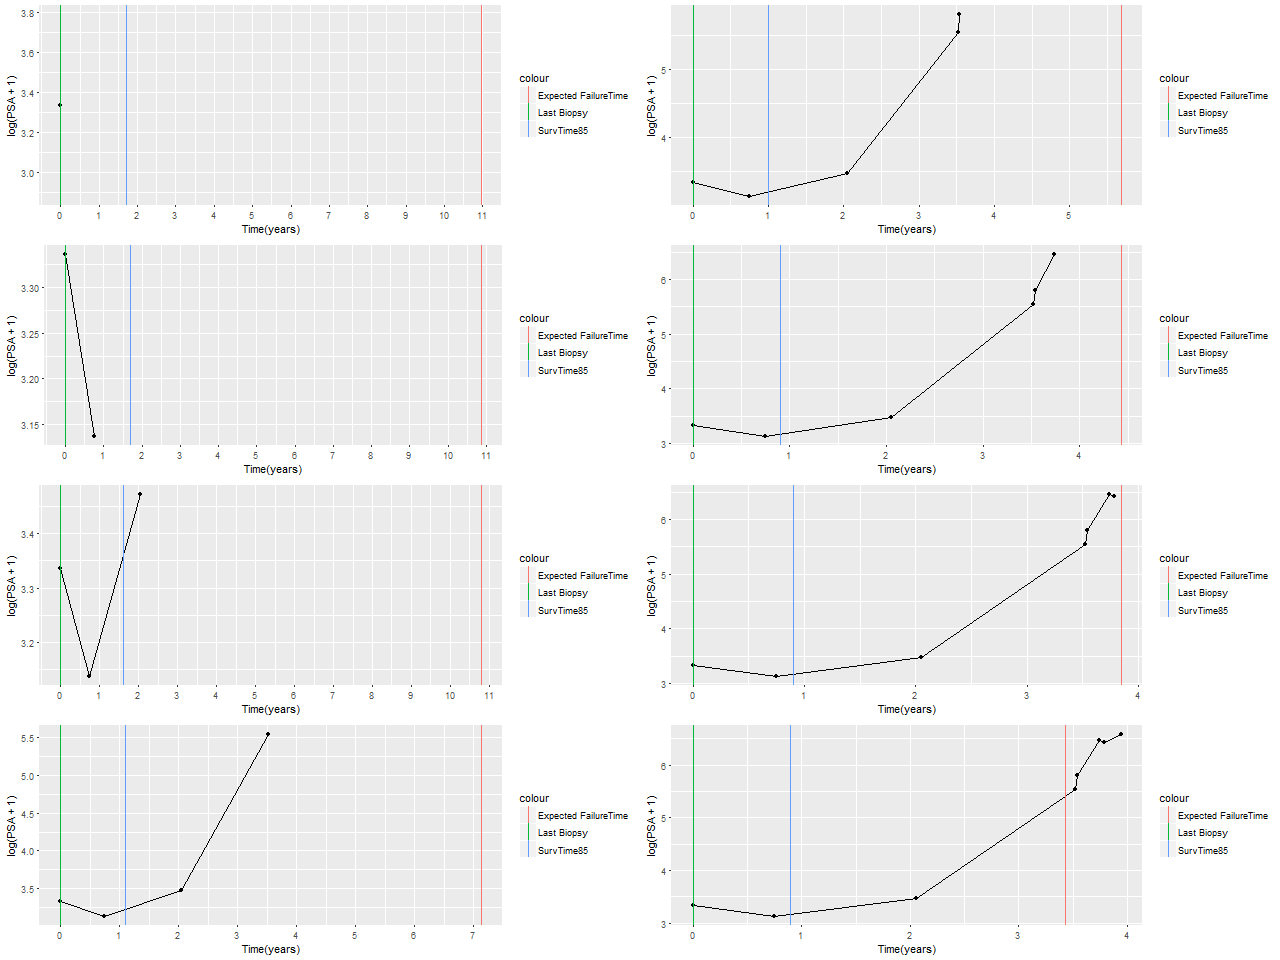
\includegraphics[width=\textwidth]{prias_demo_pid_3174.png}
\caption{\label{fig : prias_demo_pid_3174} Proposed biopsy times for patient 3174 from PRIAS.}
\end{figure}

\begin{figure}[!htb]
\centering
\captionsetup{justification=centering}
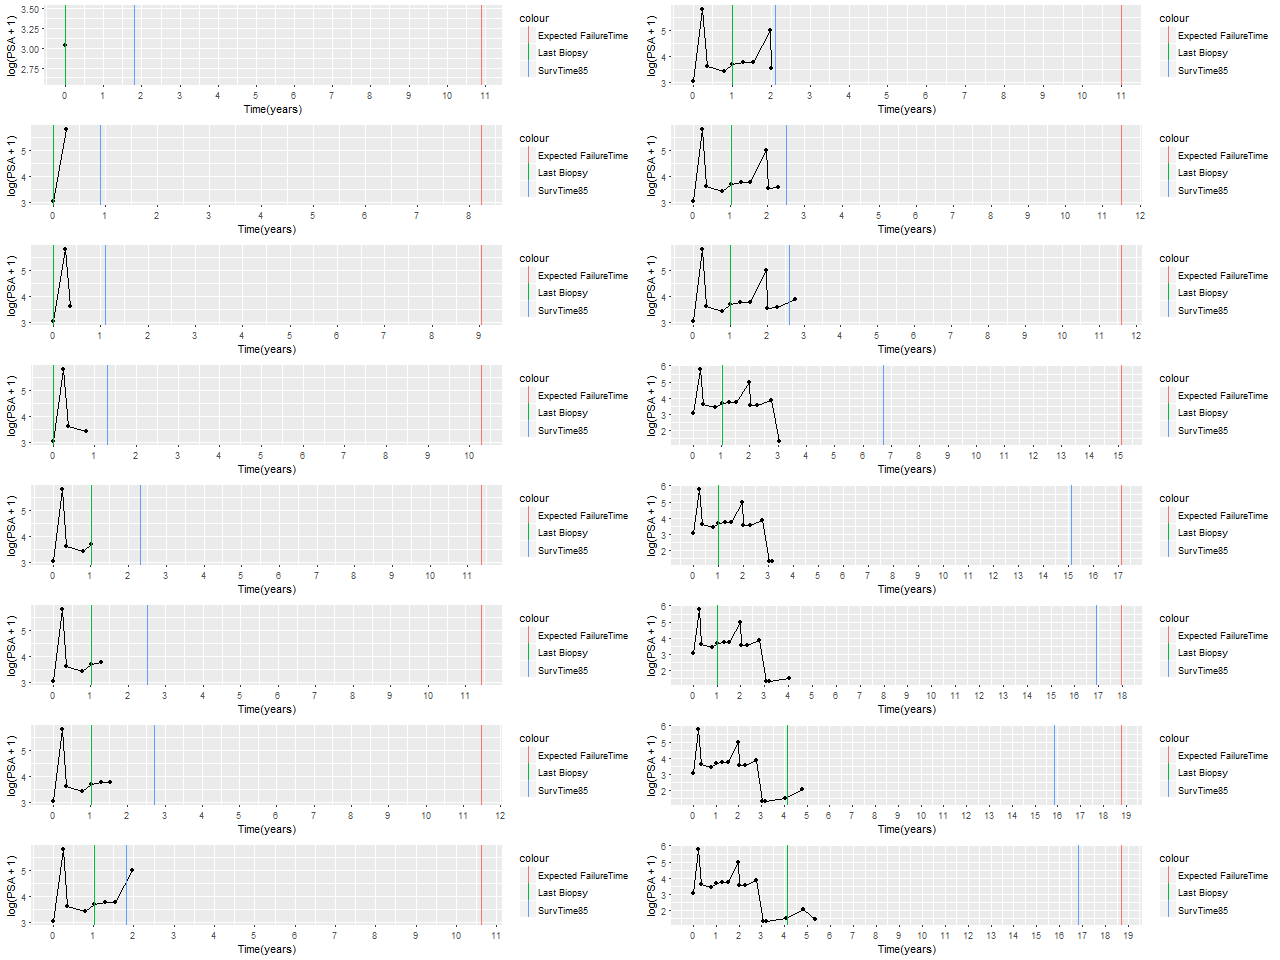
\includegraphics[width=\textwidth]{prias_demo_pid_911.png}
\caption{\label{fig : prias_demo_pid_911} Proposed biopsy times for patient 3174 from PRIAS.}
\end{figure}

\begin{figure}[!htb]
\centering
\captionsetup{justification=centering}
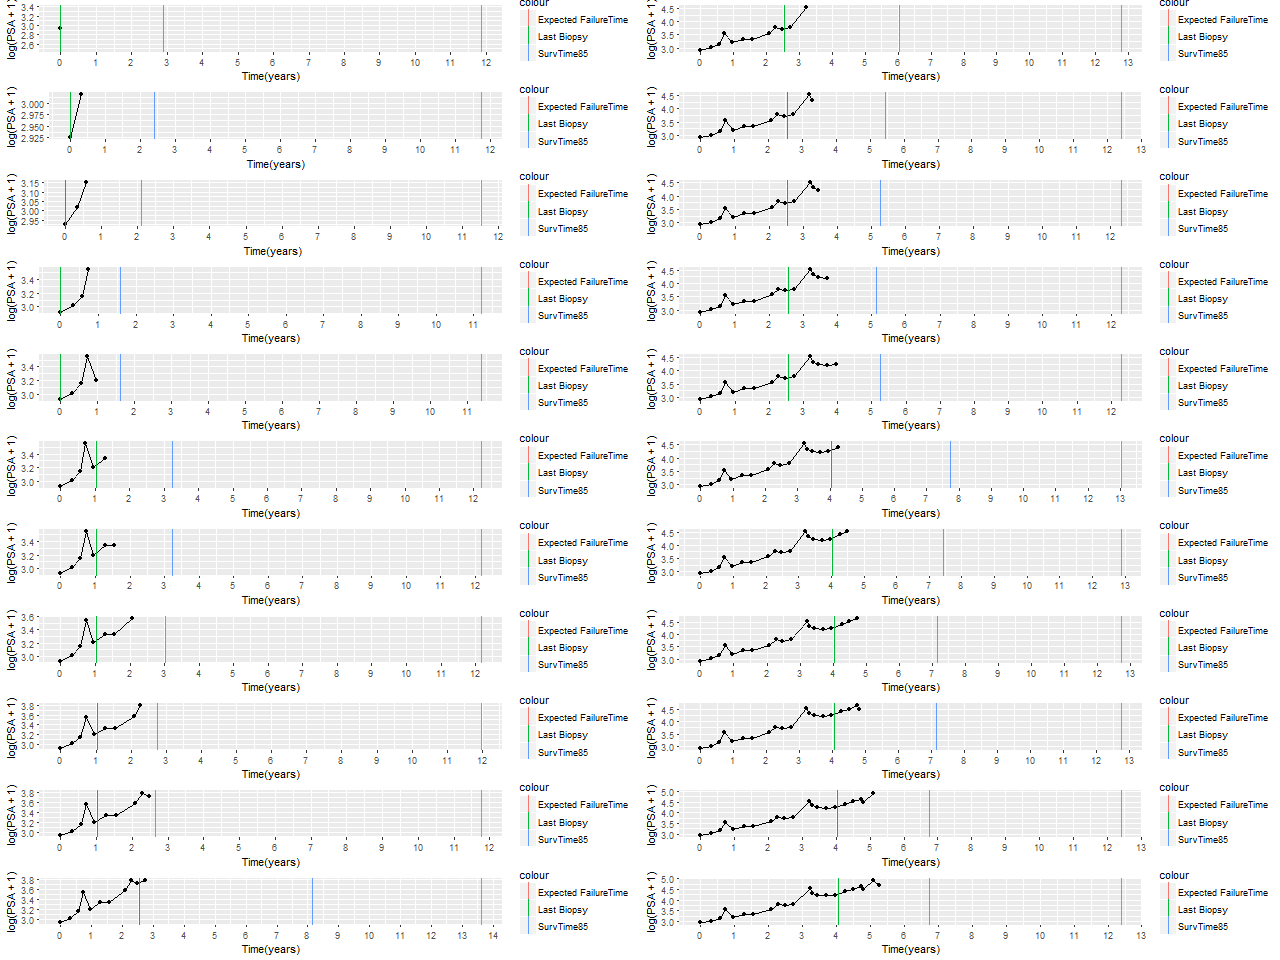
\includegraphics[width=\textwidth]{prias_demo_pid_2340.png}
\caption{\label{fig : prias_demo_pid_2340} Proposed biopsy times for patient 3174 from PRIAS.}
\end{figure}

It can be seen in Figure \ref{fig : prias_demo_pid_3174} that the patient 3174 had a biopsy at the time of induction and none after that. The PSA for the patient increases rapidly after the 2nd year. In response to this rapid increase, the proposed biopsy times based on conditional expected failure time also decrease accordingly from 11 years to around 3.4 years. The change for risk based methods is not so drastic though. Further it can be seen that at the last visit for PSA, the proposed biopsy time is earlier than the last 5 PSA visits and similar is the case for the proposed biopsy time based on dynamic risk of failure. This is due to the fact that the last time of biopsy was time 0 (induction time) and thus the time to Gleason reclassification can take any value larger than 0. We discuss this issue in detail in section \ref{subsec : simulation_setup}.\\

Figure \ref{fig : prias_demo_pid_911} shows the PSA evolution and biopsy times for subject 911. It can be seen that this patient had 3 biopsies where Gleason reclassification did not happen. At year 2 when the patient's PSA increases rapidly the proposed failure times also decrease, whereas they increase over the next 1 year because the PSA also drops down in that time period. The fact that PSA velocity affects the biopsy times the most is also evident in the case of subject 2340, whose evolution is shown in Figure \ref{fig : prias_demo_pid_2340}. Here the rate of change at each time point is not high, and even though the PSA value reaches as high as 25 it has no effect on proposed biopsy times. This is in accordance with the estimated strength of association between PSA velocity/value and hazard of time to Gleason reclassification.\\

An interesting observation we made while creating these schedules was that the variance of time to Gleason reclassification (Eq. \ref{eq : varFailureTime}) was quite high, which essentially rules out the usefulness of conditional expected time to Gleason reclassification. Given the large difference in proposed biopsy times based on the former and methods based on dynamic risk of Gleason reclassification, one might conclude that the latter are more useful. However as we will see in the simulation study (Section \ref{sec: simulation_study}) ahead, the usefulness of the two categories of methods depends on the distribution of time to Gleason reclassification.

% !TEX root =  ../main_manuscript.tex 
\section{Simulation Study}
\label{sec: simulation_study}
In Section \ref{subsec : demo_prias_pers_schedule} we demonstrated that the personalized schedules, schedule future biopsies according to the historical data of each patient. However, we could not perform a full-scale comparison between personalized and PRIAS schedules, because the true time of GR was not known for the PRIAS patients. To this end, we conducted a simulation study comparing personalized schedules with PRIAS and annual schedule, whose details are presented next.

\subsection{Simulation Setup}
\label{subsec : simulation_setup}
The population of AS patients in this simulation study is assumed to have the same entrance criteria as that of PRIAS. The PSA and hazard of GR for these patients follow a joint model of the form postulated in Section \ref{subsec : jm_fit_prias}, with parameters equal to the posterior mean of parameters estimated from the joint model fitted to the PRIAS dataset (see Web Appendix C). Furthermore, we also intend to test the efficacy of different schedules for a population which has patients with both faster as well as slowly-progressing PCa. The rate of progression is not only manifested via PSA profiles but also via the baseline hazard. We assume that there are three equal sized subgroups $G_1$, $G_2$ and $G_3$ of patients in the population, each with a baseline hazard from a Weibull distribution, with the following shape and scale parameters $(k, \lambda$): $(1.5, 4)$, $(3, 5)$ and $(4.5, 6)$ for $G_1, G_2$ and $G_3$, respectively. The effect of these parameters is that the mean GR time is lowest in $G_1$ (fast PCa progression) and highest in $G_3$ (slow PCa progression).

From this population, we have sampled 500 datasets with 1000 patients each. We generate a true GR time for each of the patients, and then sample a set of PSA measurements at the same time points as given in PRIAS protocol (see Web Appendix C). We then split the dataset into a training (750 patients) and a test (250 patients) part, and generate a random and non-informative censoring time for the training patients. We next fit a joint model of the specification given in (\ref{eq : long_model_prias}) and (\ref{eq : hazard_prias}) to each of the 500 training datasets and obtain MCMC samples from the 500 sets of the posterior distribution of the parameters. Using these fitted joint models, we obtain the posterior predictive distribution of time of GR for each of the $500 \times 250$ test patients. This distribution is further used to create personalized biopsy schedules for the test patients. For every test patient we conduct hypothetical biopsies using the following six types of schedules (abbreviated names in parenthesis): personalized schedules based on expected time of GR (Exp. GR time) and median time of GR (Med. GR time), personalized schedules based on dynamic risk of GR (Dyn. risk GR), a hybrid approach between median time of GR and dynamic risk of GR (Hybrid), PRIAS schedule and the annual schedule. The biopsies are conducted as per the algorithm in Figure \ref{fig : sched_algorithm}. 

To compare the aforementioned schedules we require estimates of the various measures of efficacy described in Section \ref{sec : choosing_schedule}. To this end, for schedule $S$, we compute pooled estimates of mean offset $E(O^S_j)$ and variance of offset $\mbox{var}(O^S_j)$, as below (estimates for $N^S_j$ are similar):
\begin{align*}
\widehat{E(O^S_j)} &= \frac{\sum_{k=1}^{500} n_k \widehat{E(O^S_k)}}{\sum_{k=1}^{500} n_k}, \\
\widehat{\mbox{var}(O^S_j)} &= \frac{\sum_{k=1}^{500} (n_k - 1) \widehat{\mbox{var}(O^S_k)}}{\sum_{k=1}^{500} (n_k-1)}, 
\end{align*}
where $n_k$ denotes the number of test patients, $\widehat{E(O^S_k)} = {\sum_{l=1}^{n_k}O^S_{kl}}/{n_k}$ is the estimated mean and $\widehat{\mbox{var}(O^S_k)} = {\sum_{l=1}^{n_k}\big\{O^S_{kl} - \widehat{E(O^S_k)}\big\}^2}/(n_k-1)$ is the estimated variance of the offset for the $k$-th simulation. The offset for the $l$-th test patient of the $k$-th dataset is denoted by $O^S_{kl}$.

\subsection{Results}
The pooled estimates of the aforementioned measures are summarized in Table \ref{table : sim_study_pooled_estimates}. In addition, estimated values of $E(O^S_j)$ are plotted against $E(N^S_j)$ in Figure \ref{fig : meanNbVsOffset}. The figure shows that across the schedules there is an inverse relationship between number $E(O^S_j)$ and $E(N^S_j)$. For example, the annual schedule conducts on average 5.2 biopsies to detect GR, which is the highest among all schedules. However, it has the least average offset of 6 months as well. On the other hand, the schedule based on expected time of GR conducts only 1.9 biopsies on average to detect GR, the least among all schedules, but it also has the highest average offset of 15 months (similar for median time of GR). Since the annual schedule attempts to contain the offset within a year it has the least $\mbox{SD}(O^S_j) = \sqrt{\mbox{var}(O^S_j)}$. However to achieve this, it conducts a wide range of number of biopsies from patient to patient, i.e., highest $\mbox{SD}(N^S_j) = \sqrt{\mbox{var}(N^S_j)}$. In this regard, schedules based on expected and median time of GR perform the opposite of annual schedule.

\begin{figure}
\centerline{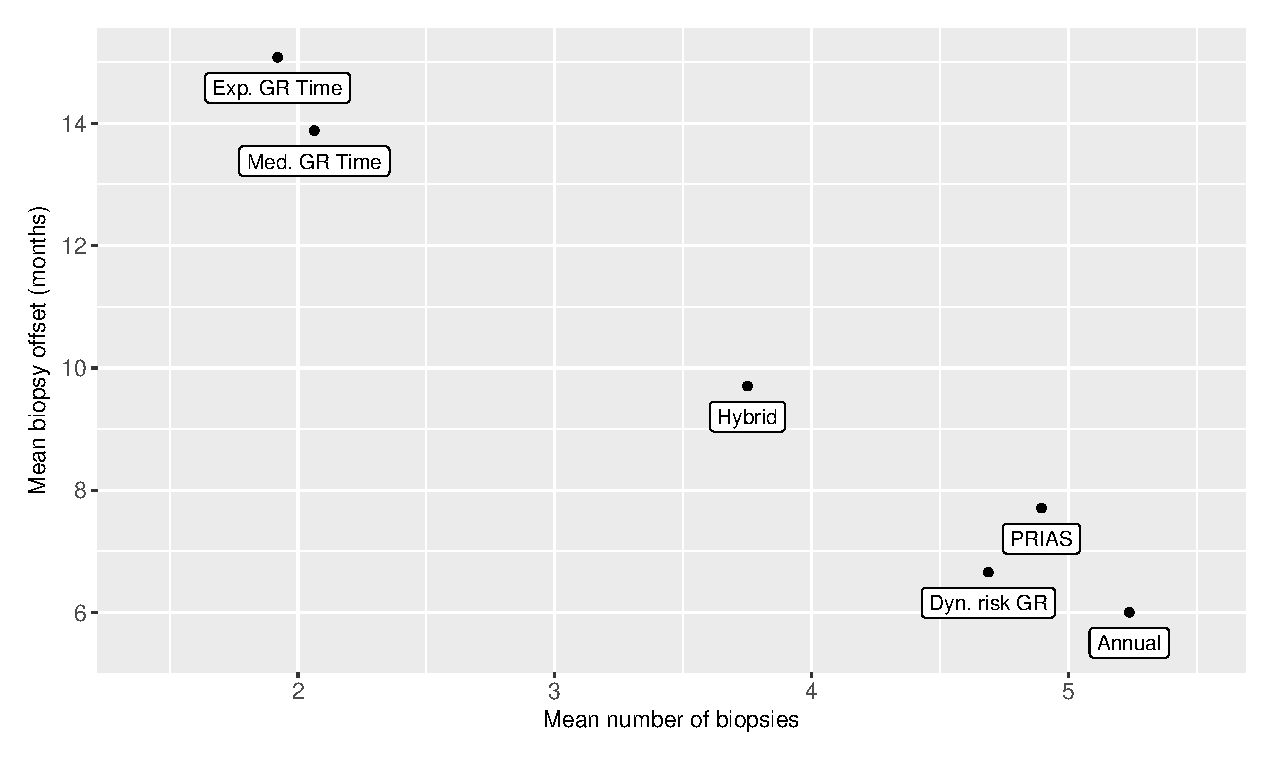
\includegraphics[width=\columnwidth]{images/sim_study/meanNbVsOffset_all.eps}}
\caption{Estimated mean number of biopsies and mean offset (months) for various schedules, obtained from the simulation study with 500 simulated datasets.}
\label{fig : meanNbVsOffset}
\end{figure}

%124781 = 41484 + 41423 + 41874
\begin{table}
\caption{Estimated mean and standard deviation of the number of biopsies $N^S_j$ and offset $O^S_j$ (months) for various schedules, obtained from the simulation study with 500 simulated datasets.}
\label{table : sim_study_pooled_estimates}
\begin{tabular}{lrrrr}
\Hline
\multicolumn{5}{c}{a) All hypothetical subgroups}\\
\hline
Schedule          & $E(N^S_j)$ & $E(O^S_j)$ & ${\mbox{SD}(N^S_j)}$ & ${\mbox{SD}(O^S_j)}$ \\
\hline
Annual         & 5.24            & 6.01                & 2.53          & 3.46              \\
PRIAS          & 4.90            & 7.71                & 2.36          & 6.31\\
Dyn. risk GR       & 4.69            & 6.66                & 2.19           & 4.38              \\
Hybrid       & 3.75            & 9.70                & 1.71          & 7.25              \\
Med. GR time & 2.06            & 13.88               & 1.41          & 11.80              \\
Exp. GR time & 1.92            & 15.08               & 1.19          & 12.11             \\
\hline
\multicolumn{5}{c}{b) Hypothetical subgroup $G_1$}\\
\hline
Schedule        & $E(N^S_j)$ & $E(O^S_j)$ & ${\mbox{SD}(N^S_j)}$ & ${\mbox{SD}(O^S_j)}$ \\
\hline
Annual         & 4.32            & 6.02                & 3.13          & 3.44              \\
PRIAS          & 4.07            & 7.44                & 2.88          & 6.11    \\
Dyn. risk GR       & 3.85            & 6.75                & 2.69          & 4.44              \\
Hybrid       & 3.25            & 10.25               & 2.16          & 8.07              \\
Med. GR time & 1.84            & 20.66               & 1.76          & 14.62             \\
Exp. GR time & 1.72            & 21.65               & 1.47          & 14.75             \\
\hline      
\multicolumn{5}{c}{c) Hypothetical subgroup $G_2$}\\
\hline
Schedule        & $E(N^S_j)$ & $E(O^S_j)$ & ${\mbox{SD}(N^S_j)}$ & ${\mbox{SD}(O^S_j)}$ \\
\hline
Annual         & 5.18            & 5.98                & 2.13          & 3.47              \\
PRIAS          & 4.85            & 7.70                & 2.00          & 6.29        \\
Dyn. risk GR       & 4.63            & 6.66                & 1.82          & 4.37              \\
Hybrid       & 3.68            & 10.32                & 1.37          & 7.45              \\
Med. GR time & 1.89             & 12.33               & 1.16          & 9.44              \\
Exp. GR time & 1.77            & 13.54               & 0.98          & 9.83              \\
\hline      
\multicolumn{5}{c}{d) Hypothetical subgroup $G_3$}\\
\hline
Schedule        & $E(N^S_j)$ & $E(O^S_j)$ & ${\mbox{SD}(N^S_j)}$ & ${\mbox{SD}(O^S_j)}$ \\
\hline
Annual         & 6.20             & 6.02                & 1.76          & 3.46              \\
PRIAS          & 5.76             & 7.98                & 1.71         & 6.51        \\
Dyn. risk GR       & 5.58            & 6.58                & 1.56          & 4.33              \\
Hybrid       & 4.32            & 8.55                & 1.26          & 5.91              \\
Med. GR time & 2.45            & 8.70                & 1.15          & 6.32              \\
Exp. GR time & 2.27            & 10.09               & 0.99          & 7.47              \\
\hline     
\end{tabular}
\end{table}

The PRIAS schedule conducts only 0.3 biopsies less than the annual schedule, but with a higher $\mbox{SD}(O^S_j)$, early detection is not always guaranteed. In comparison, the dynamic risk of GR based schedule performs slightly better than the PRIAS schedule in all four criteria. The hybrid approach combines the benefits of methods with low $E(N^S_j)$ and $\mbox{SD}(N^S_j)$, and methods with low $E(O^S_j)$ and $\mbox{SD}(O^S_j)$. It conducts 1.5 biopsies less than the annual schedule on average and with a $E(O^S_j)$ of 9.7 months it detects GR within a year since its occurrence. Moreover, it has both $\mbox{SD}(N^S_j)$ and $\mbox{SD}(O^S_j)$ comparable to PRIAS.

The performance of each schedule differs for the three subgroups $G_1, G_2$ and $G_3$. The annual schedule remains the most consistent across subgroups in terms of the offset, but it conducts 2 extra biopsies for the subgroup $G_3$ (slowly-progressing PCa) than $G_1$ (faster-progressing PCa). The performance of schedule based on expected time of GR is the most consistent in terms of the number of biopsies but it detects GR a year later on average in subgroup $G_1$ than $G_3$. For the dynamic risk of GR based schedule and the hybrid schedule, the dynamics are similar to that of the annual schedule. Unlike the latter two schedules, the PRIAS schedule not only conducts more biopsies in $G_3$ than $G_1$ but also detects GR later in $G_3$ than $G_1$.

\begin{figure}[!htb]
\centerline{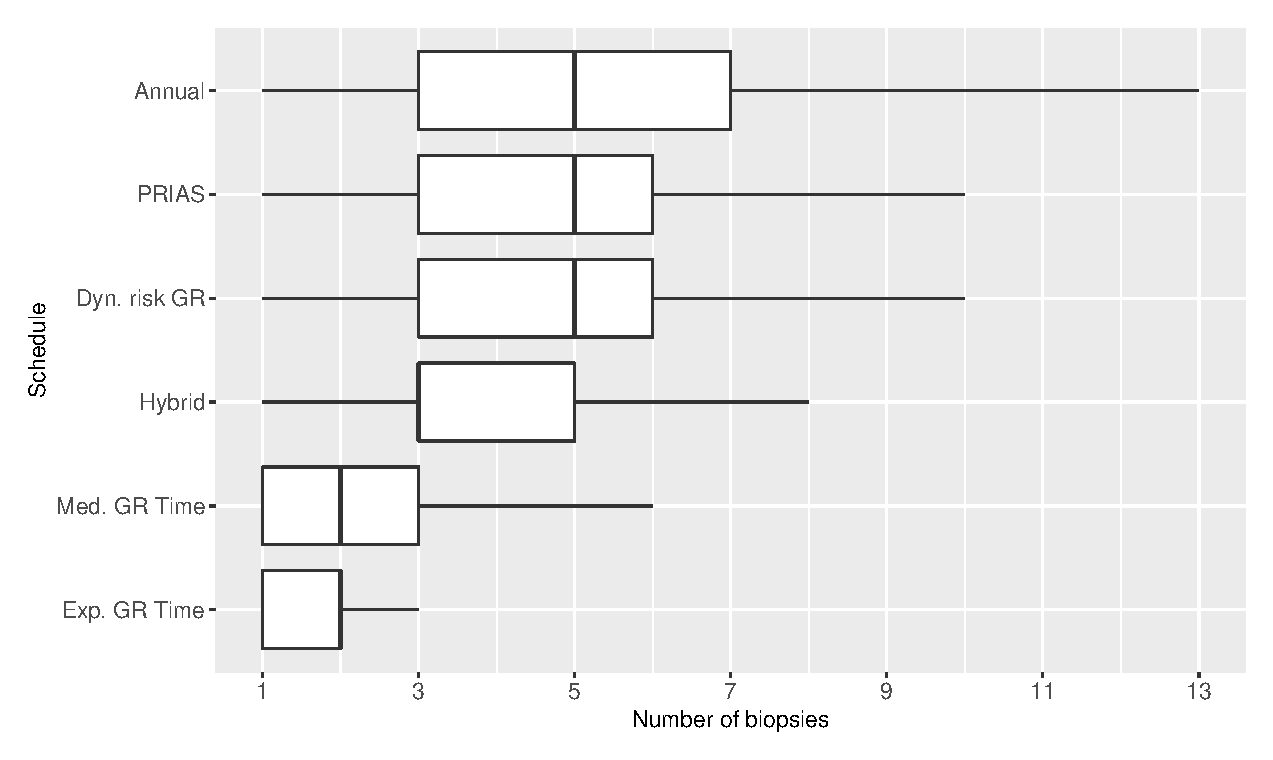
\includegraphics[width=\columnwidth]{images/sim_study/nbBoxPlot_all.eps}}
\caption{Boxplot showing variation in number of biopsies conducted by various schedules, obtained from the simulation study with 500 simulated datasets.}
\label{fig : nbBoxPlot_all}
\end{figure}

\begin{figure}[!htb]
\centerline{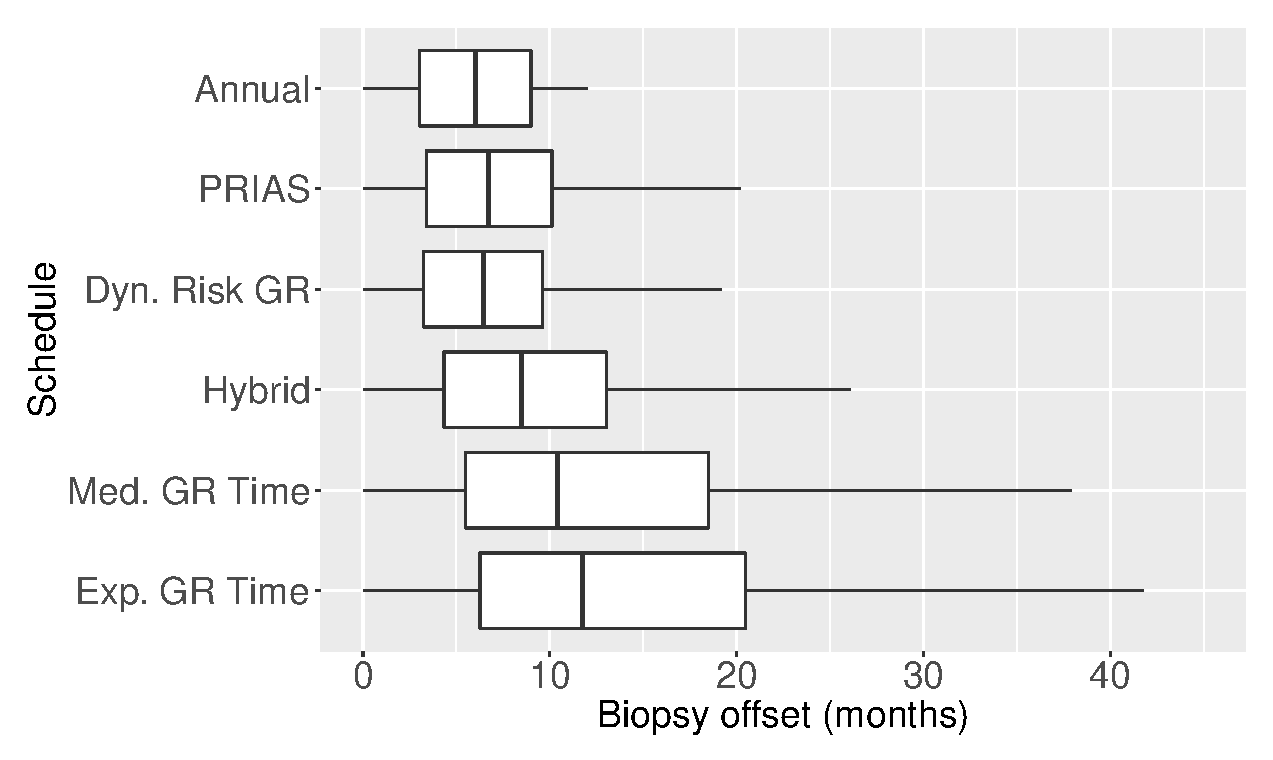
\includegraphics[width=\columnwidth]{images/sim_study/offsetBoxPlot_all.eps}}
\caption{Boxplot showing variation in biopsy offset (months) for various schedules, obtained from the simulation study with 500 simulated datasets.}
\label{fig : offsetBoxPlot_all}
\end{figure}

The choice of a suitable schedule using (\ref{eq : loss_func_sim_study_generic}) depends on the chosen measure for evaluation of schedules. In this regard, the schedules we compared either have high $\mbox{SD}(O^S_j)$ and low $\mbox{SD}(N^S_j)$, or vice versa (Table \ref{table : sim_study_pooled_estimates}). Thus, applying a cutoff on $E(O^S_j)$ when $\mbox{SD}(O^S_j)$ is high may not be as fruitful (same for $N^S_j$) as applying a cutoff on $\mbox{SD}(O^S_j)$ or quantile(s) of $O^S_j$. For example, the schedule based on the dynamic risk of GR is suitable if on average the least number of biopsies are to be conducted to detect GR, while simultaneously making sure that at least 90\% of the patients have an average offset less than one year.


\textbf{}

\clearpage
\printbibliography

\appendix

% !TEX root =  ../main.tex 

\section{Appendix}

\subsection{Personalized schedules for repeat biopsies}
In this section we present the derivations for Equation \ref{eq : expected_time_survprob} and Equation \ref{eq : var_time_survprob}. To this end, we first expand the formula for dynamic survival probability presented in Equation \ref{eq : dynamic_surv_prob}.
\begin{equation}
\label{eq : dyn_surv_prob_expanded}
\begin{split}
\pi_j(u \mid t, s) &= \mbox{Pr}\big\{T^*_j \geq u \mid  T^*_j >t, \mathcal{Y}_j(s\big\}, D_n)\\
&= \int \int \mbox{Pr}\big\{T^*_j \geq u \mid  T^*_j >t, \boldsymbol{b}_j,\boldsymbol{\theta}\big\} p\big(\boldsymbol{b}_j \mid T^*_j>t, \mathcal{Y}_j(s), \boldsymbol{\theta}\big)p\big(\boldsymbol{\theta} \mid \mathcal{D}_n\big) \diff \boldsymbol{b}_j \diff \boldsymbol{\theta}\\
&= \int \int \frac{\exp\big\{-H_j(u | \boldsymbol{b}_j, \boldsymbol{\theta})\big\}}{\exp\big\{-H_j(t | \boldsymbol{b}_j, \boldsymbol{\theta})\big\}} p\big(\boldsymbol{b}_j \mid T^*_j>t, \mathcal{Y}_j(s), \boldsymbol{\theta}\big)p\big(\boldsymbol{\theta} \mid \mathcal{D}_n\big) \diff \boldsymbol{b}_j \diff \boldsymbol{\theta}
\end{split}
\end{equation}
where $H_j(u | \boldsymbol{b}_j, \boldsymbol{\theta}) = \int_0^u h_i(s \mid \boldsymbol{b}_j, \boldsymbol{\theta}\big)\diff s$ is the cumulative hazard up to time point $u$.

\subsubsection{Derivation of Equation \ref{eq : expected_time_survprob}}
\label{subsubsec : deriv_eq_7}
\begin{equation*}
\begin{split}
E_g[T^*_j] &= \int_t^{\infty} T^*_j g(T^*_j)\diff T^*_j\\
\text{Using integration by parts, wherein} & \frac{\diff \big\{-\pi_j(T^*_j \mid t, s)\big\}}{\diff T^*_j} = g(T^*_j)\\
&= \Big[-T^*_j\pi_j(T^*_j \mid t, s)\Big]_t^\infty + \int_t^{\infty} \pi_j(T^*_j \mid t, s) \frac{\diff (T^*_j)}{\diff T^*_j} \diff T^*_j\\
&= t \pi_j(t \mid t, s) - \lim_{T^*_j\to \infty}T^*_j \pi_j(T^*_j \mid t, s) + \int_t^{\infty} \pi_j(T^*_j \mid t, s) \diff T^*_j\\
\end{split}
\end{equation*}
where $\pi_j(t \mid t, s) = \mbox{Pr}\big\{T^*_j \geq t \mid  T^*_j >t, \mathcal{Y}_j(s), D_n\big\} = 1$. As for $\lim_{T^*_j\to \infty}T^*_j \pi_j(T^*_j \mid t, s)$, the limit can be interchanged with the integral in Equation \ref{eq : dyn_surv_prob_expanded}, because as $T^*_j\to \infty$ the integrand in the equation converges uniformly on the domain of $(\boldsymbol{b}_j, \boldsymbol{\theta}\big)$. Thus,
\begin{equation*}
\begin{split}
\lim_{T^*_j\to \infty}T^*_j \pi_j(T^*_j \mid t, s) &=  \int \int \lim_{T^*_j\to \infty} \frac{T^*_j}{\exp\big\{H_j(T^*_j | \boldsymbol{b}_j, \boldsymbol{\theta})\big\}} \frac{p\big(\boldsymbol{b}_j \mid T^*_j>t, \mathcal{Y}_j(s), \boldsymbol{\theta}\big)p\big(\boldsymbol{\theta} \mid \mathcal{D}_n\big)}{\exp\big\{-H_j(t | \boldsymbol{b}_j, \boldsymbol{\theta})\big\}}  \diff \boldsymbol{b}_j \diff \boldsymbol{\theta}\\
\text{Using L'Hospital's rule}\\
\lim_{T^*_j\to \infty}T^*_j \pi_j(T^*_j \mid t, s) &=  \int \int \frac{1}{\lim_{T^*_j\to \infty} \exp\{H_j(T^*_j | \boldsymbol{b}_j, \boldsymbol{\theta}\big)\}H'_j(T^*_j | \boldsymbol{b}_j, \boldsymbol{\theta}\big)} \frac{p\big(\boldsymbol{b}_j \mid T^*_j>t, \mathcal{Y}_j(s), \boldsymbol{\theta}\big)p\big(\boldsymbol{\theta} \mid \mathcal{D}_n\big)}{\exp\{-H_j(t | \boldsymbol{b}_j, \boldsymbol{\theta}\big)\}} \diff \boldsymbol{b}_j \diff \boldsymbol{\theta}\\
&= \int \int 0 \frac{p\big(\boldsymbol{b}_j \mid T^*_j>t, \mathcal{Y}_j(s), \boldsymbol{\theta}\big)p\big(\boldsymbol{\theta} \mid \mathcal{D}_n\big)}{\exp\big\{-H_j(t | \boldsymbol{b}_j, \boldsymbol{\theta})\big\}}  \diff \boldsymbol{b}_j \diff \boldsymbol{\theta}\\
&= 0
\end{split}
\end{equation*}

In light of these results, we obtain:
\begin{equation*}
E_g[T^*_j] = t + \int_t^{\infty} \pi_j(T^*_j \mid t, s) \diff T^*_j\\
\end{equation*}

\subsubsection{Derivation of Equation \ref{eq : var_time_survprob}}
Since $\mbox{var}_g[T^*_j] = E_g[\{T^*_j\}^2] - E_g[T^*_j]^2$, we first show the derivation for $E_g[(T^*_j)^2]$.
\begin{equation*}
\begin{split}
E_g[(T^*_j)^2] &= \int_t^{\infty} (T^*_j)^2 g(T^*_j)\diff T^*_j\\
\text{Using integration by parts, wherein} & \frac{\diff \big\{-\pi_j(T^*_j \mid t, s)\big\}}{\diff T^*_j} = g(T^*_j)\\
E_g\big[\{T^*_j\}^2\big] &= \Big[-\{T^*_j\}^2\pi_j(T^*_j \mid t, s)\Big]_t^\infty + \int_t^{\infty} \pi_j(T^*_j \mid t, s) \frac{\diff (T^*_j)^2}{\diff T^*_j} \diff T^*_j\\
&= t^2 \pi_j(t \mid t, s) - \lim_{T^*_j\to \infty}(T^*_j)^2 \pi_j(T^*_j \mid t, s) + 2 \int_t^{\infty} T^*_j \pi_j(T^*_j \mid t, s) \diff T^*_j\\
&= t^2 + 2 \int_t^{\infty} T^*_j \pi_j(T^*_j \mid t, s) \diff T^*_j
\end{split}
\end{equation*}
Therefore,
\begin{equation*}
\begin{split}
\mbox{var}_g[T^*_j] &= t^2 + 2 \int_t^{\infty} T^*_j \pi_j(T^*_j \mid t, s) \diff T^*_j - \bigg[t^2 +  \Big\{\int_t^\infty \pi_j(T^*_j \mid t, s) \diff T^*_j \Big\}^2 + 2t\int_t^\infty \pi_j(T^*_j \mid t, s) \diff T^*_j \bigg]\\
&=2 \int_t^{\infty} (T^*_j - t) \pi_j(T^*_j \mid t, s) \diff T^*_j -  \Big\{\int_t^\infty \pi_j(T^*_j \mid t, s) \diff T^*_j \Big\}^2
\end{split}
\end{equation*}

\subsection{Simulation study}
This section presents the figures and tables for related to the simulation study results from Section \ref{sec: simulation_study}. More specifically:

\begin{itemize}
  \item Figure \ref{fig : meanNbVsOffset_G1}, Figure \ref{fig : meanNbVsOffset_G2} and Figure \ref{fig : meanNbVsOffset_G3} show plots of average number of biopsies against average offset for each of the 7 scheduling methods present in the simulation study.
  \item Figure \ref{fig : nbBoxPlot_G1} and Figure \ref{fig : offsetBoxPlot_G1} show boxplots of number of biopsies and offset for each of the 6 scheduling methods for the patients in subgroup $G_1$. Similar plots for subgroup $G_2$ and $G_3$ are shown in Figure \ref{fig : nbAndOffsetBoxPlot_G2} and Figure \ref{fig : nbAndOffsetBoxPlot_G3} respectively.
  \item Figure \ref{fig : nbMeanBoxPlot_all} and Figure \ref{fig : offsetMeanBoxPlot_all} show the variation in estimated mean number of biopsies and estimated mean offset computed during the 254 simulations, for patients from all subgroups. The same plots for each of the subgroups are shown in Figure \ref{fig : nbAndOffsetMeanBoxPlot_G1}, Figure \ref{fig : nbAndOffsetMeanBoxPlot_G2} and Figure \ref{fig : nbAndOffsetMeanBoxPlot_G3}.
\end{itemize} 

\begin{figure}[!htb]
    \centering
    \captionsetup{justification=centering}
     \begin{subfigure}[b]{0.45\textwidth}
        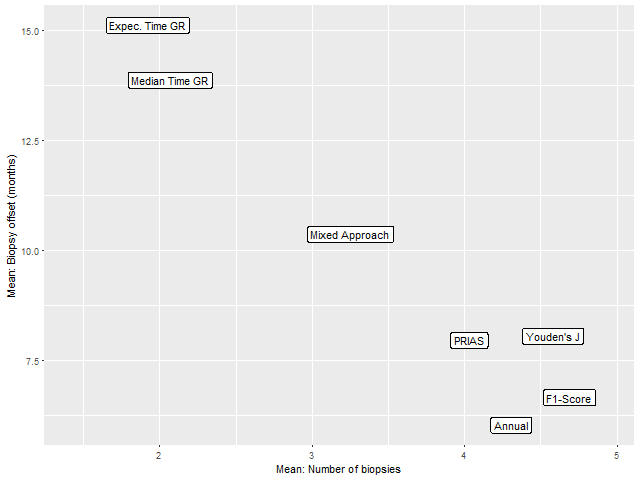
\includegraphics[width=\textwidth]{images/sim_study/meanNbVsOffset_scale_4.png}
		\caption{Plot for subgroup $G_1$}
		\label{fig : meanNbVsOffset_G1}
    \end{subfigure}
    \begin{subfigure}[b]{0.45\textwidth}
		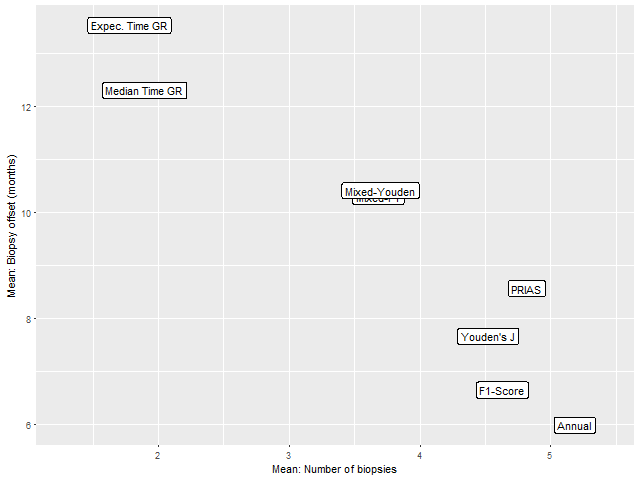
\includegraphics[width=\textwidth]{images/sim_study/meanNbVsOffset_scale_5.png}
		\caption{Plot for subgroup $G_2$}
		\label{fig : meanNbVsOffset_G2}
    \end{subfigure}  
    \begin{subfigure}[b]{0.45\textwidth}
		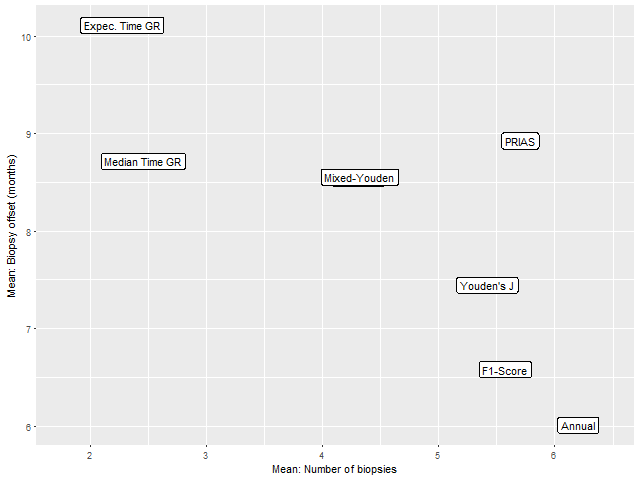
\includegraphics[width=\textwidth]{images/sim_study/meanNbVsOffset_scale_6.png}
		\caption{Plot for subgroup $G_3$}
		\label{fig : meanNbVsOffset_G3}
    \end{subfigure}      
    \caption{Estimated mean number of biopsies and mean offset (months) for the 7 scheduling methods for the 3 sub-groups. Method names are abbreviated for ease of graphing.}
\end{figure}

\begin{figure}[!htb]
    \centering
    \captionsetup{justification=centering}
     \begin{subfigure}[b]{0.45\textwidth}
        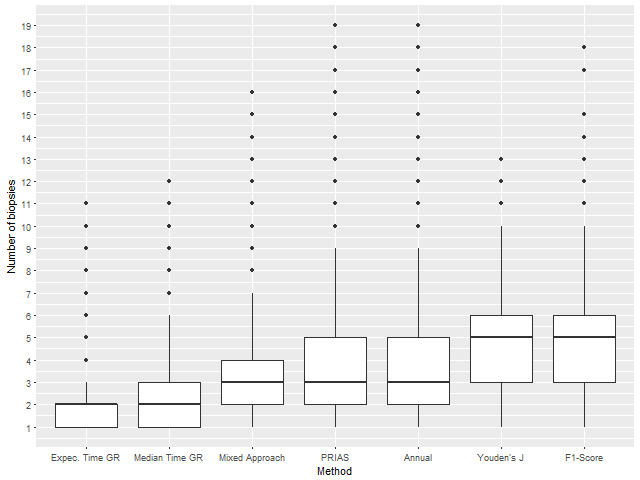
\includegraphics[width=\textwidth]{images/sim_study/nbBoxPlot_scale_4.png}
        \caption{Boxplot for number of biopsies.}
        \label{fig : nbBoxPlot_G1}
    \end{subfigure}
    \begin{subfigure}[b]{0.45\textwidth}
        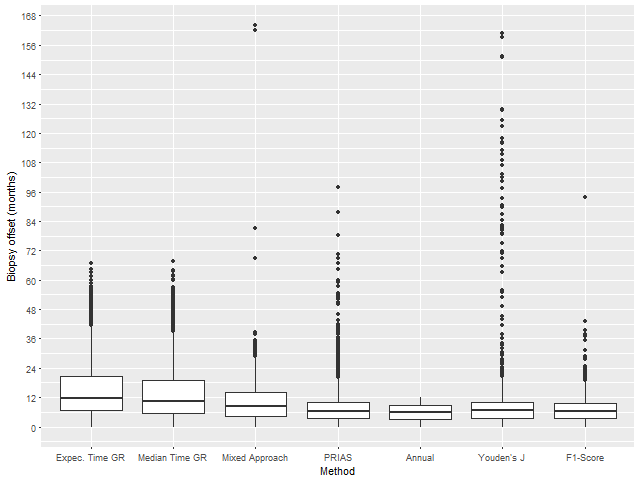
\includegraphics[width=\textwidth]{images/sim_study/offsetBoxPlot_scale_4.png}
        \caption{Boxplot for offset (months)}
        \label{fig : offsetBoxPlot_G1}
    \end{subfigure}      
    \caption{Boxplot for number of biopsies and offset (months), for all patients in subgroup $G_1$ across all simulations. Method names are abbreviated for ease of graphing.}
    \label{fig : nbAndOffsetBoxPlot_G1}
\end{figure}

\begin{figure}[!htb]
    \centering
    \captionsetup{justification=centering}
     \begin{subfigure}[b]{0.45\textwidth}
        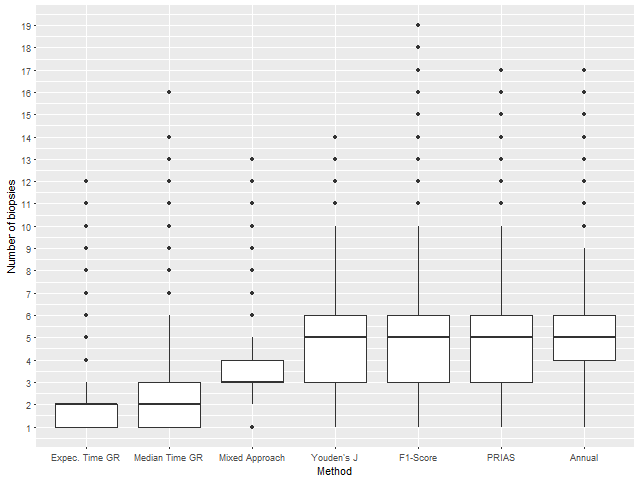
\includegraphics[width=\textwidth]{images/sim_study/nbBoxPlot_scale_5.png}
        \caption{Boxplot for number of biopsies.}
        \label{fig : nbBoxPlot_G2}
    \end{subfigure}
    \begin{subfigure}[b]{0.45\textwidth}
        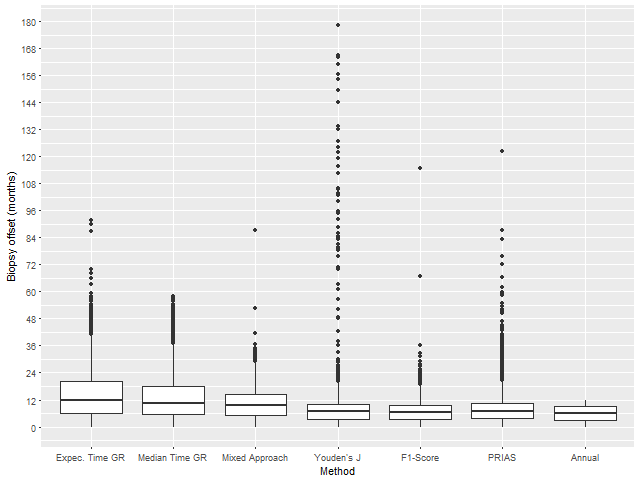
\includegraphics[width=\textwidth]{images/sim_study/offsetBoxPlot_scale_5.png}
        \caption{Boxplot for offset (months)}
        \label{fig : offsetBoxPlot_G2}
    \end{subfigure}      
    \caption{Boxplot for number of biopsies and offset (months), for all patients in subgroup $G_2$ across all simulations. Method names are abbreviated for ease of graphing.}
     \label{fig : nbAndOffsetBoxPlot_G2}
\end{figure}

\begin{figure}[!htb]
    \centering
    \captionsetup{justification=centering}
     \begin{subfigure}[b]{0.45\textwidth}
        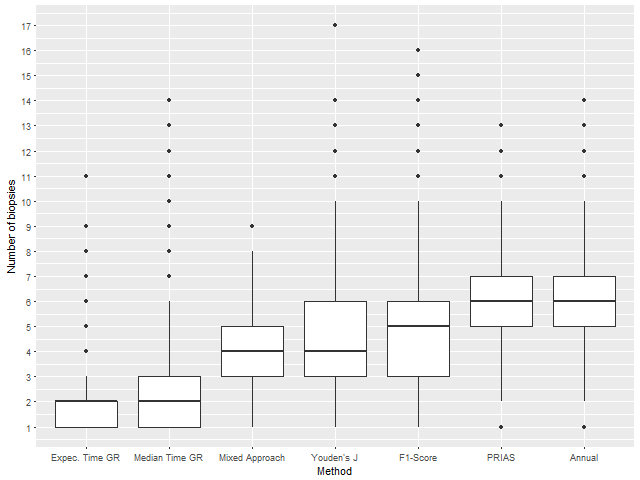
\includegraphics[width=\textwidth]{images/sim_study/nbBoxPlot_scale_6.png}
        \caption{Boxplot for number of biopsies.}
        \label{fig : nbBoxPlot_G3}
    \end{subfigure}
    \begin{subfigure}[b]{0.45\textwidth}
        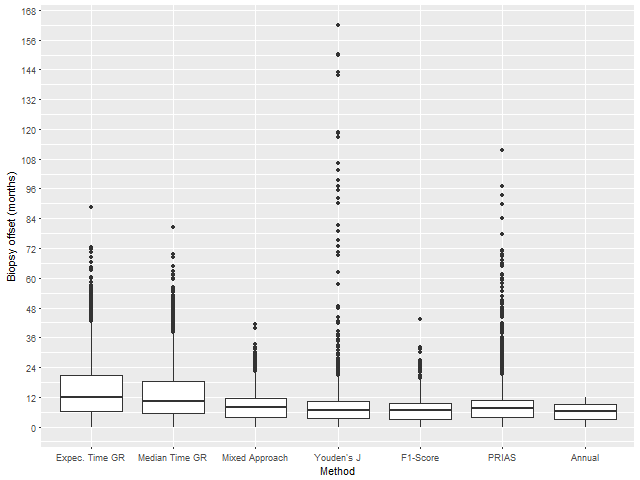
\includegraphics[width=\textwidth]{images/sim_study/offsetBoxPlot_scale_6.png}
        \caption{Boxplot for offset (months)}
        \label{fig : offsetBoxPlot_G3}
    \end{subfigure}      
    \caption{Boxplot for number of biopsies and offset (months), for all patients in subgroup $G_3$ across all simulations. Method names are abbreviated for ease of graphing.}
     \label{fig : nbAndOffsetBoxPlot_G3}
\end{figure}

\begin{figure}[!htb]
    \centering
    \captionsetup{justification=centering}
     \begin{subfigure}[b]{0.45\textwidth}
        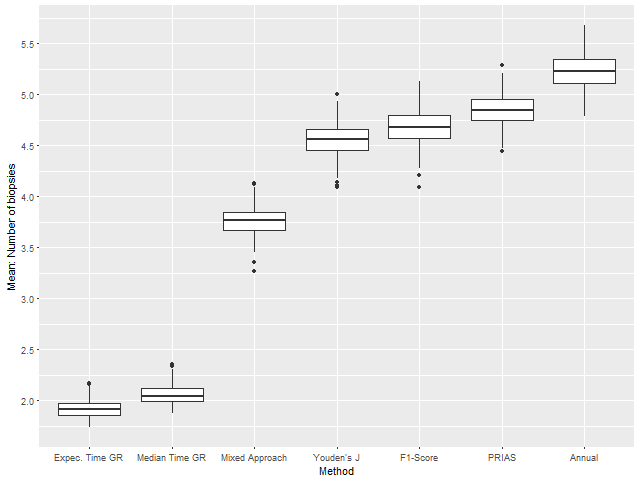
\includegraphics[width=\textwidth]{images/sim_study/nbMeanBoxPlot_all.png}
        \caption{Boxplot for mean number of biopsies.}
        \label{fig : nbMeanBoxPlot_all}
    \end{subfigure}
    \begin{subfigure}[b]{0.45\textwidth}
        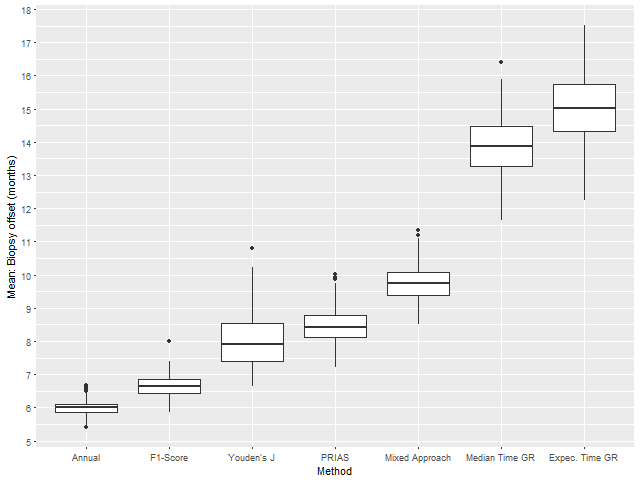
\includegraphics[width=\textwidth]{images/sim_study/offsetMeanBoxPlot_all.png}
        \caption{Boxplot for mean offset (months)}
        \label{fig : offsetMeanBoxPlot_all}
    \end{subfigure}      
    \caption{Boxplot showing variation in mean number of biopsies and mean offset (months) for all of the patients across the 254 simulations.}
\end{figure}

\begin{figure}[!htb]
    \centering
    \captionsetup{justification=centering}
     \begin{subfigure}[b]{0.45\textwidth}
        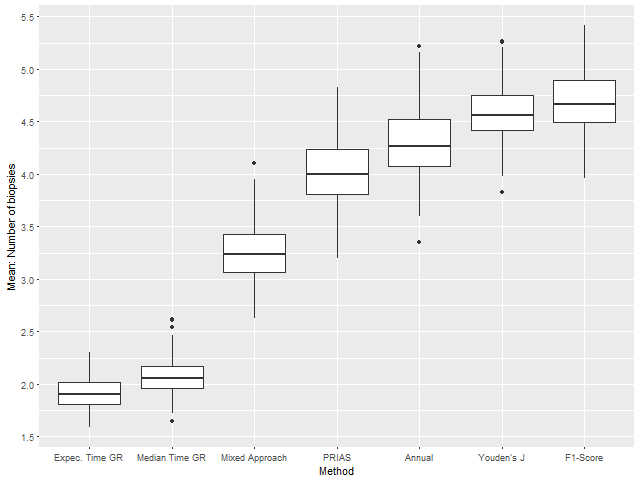
\includegraphics[width=\textwidth]{images/sim_study/nbMeanBoxPlot_scale_4.png}
        \caption{Boxplot for mean number of biopsies.}
        \label{fig : nbMeanBoxPlot_G1}
    \end{subfigure}
    \begin{subfigure}[b]{0.45\textwidth}
        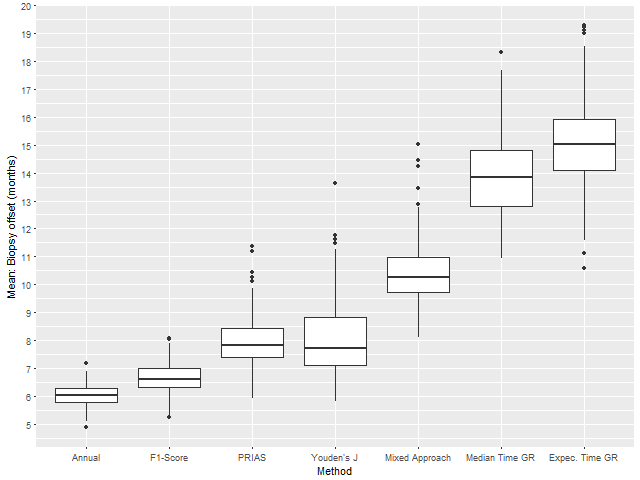
\includegraphics[width=\textwidth]{images/sim_study/offsetMeanBoxPlot_scale_4.png}
        \caption{Boxplot for mean offset (months)}
        \label{fig : offsetMeanBoxPlot_G1}
    \end{subfigure}      
    \caption{Boxplot showing variation in mean number of biopsies and mean offset (months) for patients in subgroup $G_1$ across the 254 simulations.}
    \label{fig : nbAndOffsetMeanBoxPlot_G1}
\end{figure}

\begin{figure}[!htb]
    \centering
    \captionsetup{justification=centering}
     \begin{subfigure}[b]{0.45\textwidth}
        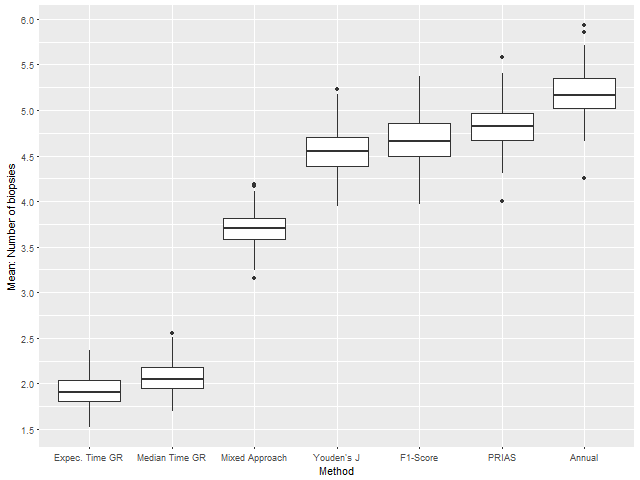
\includegraphics[width=\textwidth]{images/sim_study/nbMeanBoxPlot_scale_5.png}
        \caption{Boxplot for mean number of biopsies.}
        \label{fig : nbMeanBoxPlot_G2}
    \end{subfigure}
    \begin{subfigure}[b]{0.45\textwidth}
        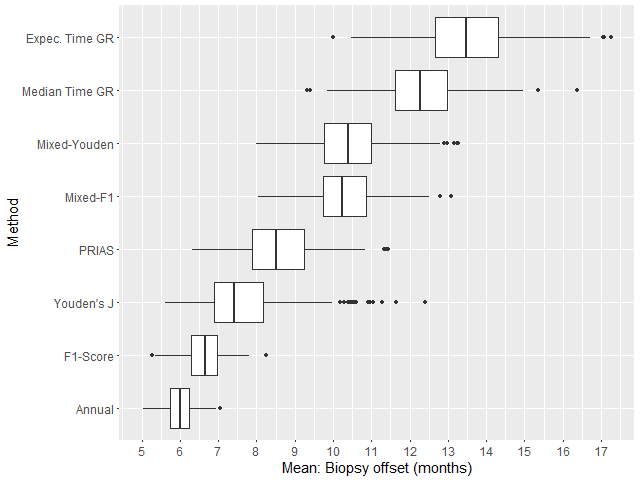
\includegraphics[width=\textwidth]{images/sim_study/offsetMeanBoxPlot_scale_5.png}
        \caption{Boxplot for mean offset (months)}
        \label{fig : offsetMeanBoxPlot_G2}
    \end{subfigure}      
    \caption{Boxplot showing variation in mean number of biopsies and mean offset (months) for patients in subgroup $G_2$ across the 254 simulations.}
    \label{fig : nbAndOffsetMeanBoxPlot_G2}
\end{figure}

\begin{figure}[!htb]
    \centering
    \captionsetup{justification=centering}
     \begin{subfigure}[b]{0.45\textwidth}
        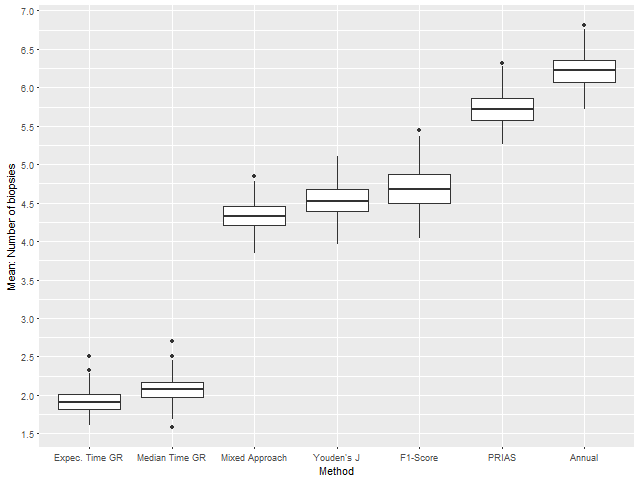
\includegraphics[width=\textwidth]{images/sim_study/nbMeanBoxPlot_scale_6.png}
        \caption{Boxplot for mean number of biopsies.}
        \label{fig : nbMeanBoxPlot_G3}
    \end{subfigure}
    \begin{subfigure}[b]{0.45\textwidth}
        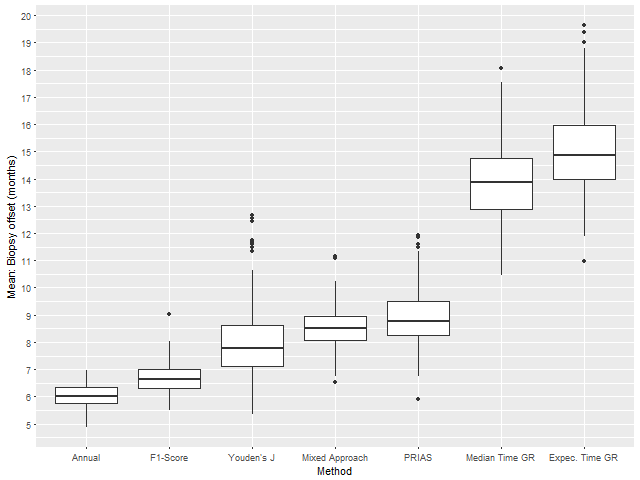
\includegraphics[width=\textwidth]{images/sim_study/offsetMeanBoxPlot_scale_6.png}
        \caption{Boxplot for mean offset (months)}
        \label{fig : offsetMeanBoxPlot_G3}
    \end{subfigure}      
    \caption{Boxplot showing variation in mean number of biopsies and mean offset (months) for patients in subgroup $G_3$ across the 254 simulations.}
    \label{fig : nbAndOffsetMeanBoxPlot_G3}
\end{figure}

\end{document}